\documentclass{article}
\usepackage{setspace}
\usepackage{natbib}
\usepackage{amsmath}
\usepackage{float}
\usepackage{longtable}
\usepackage{booktabs}
\usepackage{lscape}
\usepackage{graphicx}
\usepackage{silence}
\usepackage{forest}
\usepackage{hyperref}
\usepackage{xr}
\usepackage{placeins}
\usepackage{textcomp} % Needed on Windows in Office
\usepackage{adjustbox}
\usepackage{xcolor}
\usepackage[letterpaper, margin=1in]{geometry}

\usepackage[toc,page]{appendix}


\let\Oldsubsection\subsection
% \renewcommand{\subsection}{\FloatBarrier\Oldsubsection}
\newcommand{\comment}[1]{}

\author{Ann Atwater\footnote{Department of Economics, University of Florida.}}
\title{Maverick Firms And Competition: Evidence from the Attempted JetBlue-Spirit Merger\footnote{This is a preliminary draft. Please do not distribute without permission of the author. The author would like to thank the participants of the University of Florida Applied Microeconomics working group and of the Southern Economics Association 2024 conference for helpful feedback. Furthermore, the author would like to thank Brad Shrago for alerting her to the reliance on usage fees by ultra-low cost carriers. }}

\graphicspath{{05.Figures/}}

\begin{document}
	\maketitle
	
	\begin{abstract}
In 2024, the attempted merger between JetBlue Airways and Spirit Airlines was blocked following a lawsuit brought by the Department of Justice. This paper estimates the counterfactual effects from this merger. I find minimal impacts to average market prices under more favorable simulations and negative impacts to the average market fare of under 5\% under the worst case scenario. Furthermore, I analyze the change in the overall distribution of fares had the merger been completed. I find that even under the assumptions most favorable to pro-competitive effects from merger, I estimate that over 35 markets in both the three years before and after the pandemic would have had their minimum fares increase by over \$60. This represents a large increase in fares for highly price-conscious consumers, aligning with the judgment which prevented the merger. \bigskip

    \noindent JEL Classification: L4, L41 \newline
	\noindent Keywords: airlines; mergers; antitrust
		
	\end{abstract}
	
	\pagebreak
	
	\doublespacing
	
	\section{Introduction}
	\label{sec:Introduction} 

    

   % In 2024, a proposed merger between JetBlue and Spirit became the first merger within the American aviation sector to be blocked following trial. This merger would have seen the largest ultra-low cost carrier acquired by a low-cost carrier. Spirit had, over the course of the 2010s, pioneered the ultra-low cost carrier business model within the United States and acted as a maverick firm which competed vigorously for budget conscious travelers. As such, understanding the counterfactual effects of this merger allows for an increased understanding of the role of maverick firms in promoting competition. 
 
   % The estimation of the effects of this merger is complicated by two factors - JetBlue's Northeast Alliance (NEA) with American Airlines and the COVID-19 pandemic. Under the NEA, JetBlue and American Airlines coordinated on setting routes to and from airports serving the Boston and New York City metropolitan areas (Boston Logan International Airport, Newark Liberty International Airport, John F. Kennedy International Airport, and LaGuardia Airport) between 2020 and 2023. This agreement would be found to be anti-competitive following trial in 2023. Due to this agreement, JetBlue operated in different markets than it otherwise would have, inhibiting the understanding of the counterfactual world where the merger had been approved.

   % Concurrent with this anti-competitive conduct, the aviation industry was dealing with the ramifications of the COVID-19 pandemic on consumption patterns. While air travel levels would return to 2016 levels by the second quarter of 2021, less price-conscious business travel had dramatically decreased due to the increased prevalence of telecommunications use for meetings and has only recently recovered to pre-pandemic patterns. Leisure travelers, traditionally more price sensitive than business travelers, were observed to be behaving less price sensitively than normal by airlines, possibly owing to acquired savings during the travel slowdown.

  %  To resolve the issues presented by these factors, I estimate the counterfactual price effects of the merger on markets within the three years before the pandemic and the three years after the second quarter of 2021. While each period of analysis is separately flawed (the pre-pandemic period has normal routing but inaccurate demand patterns while the post-pandemic period has adversely impacted routing with normal demand patterns), the net picture of the merger is clear. I estimate anti-competitive price increases dominating fares at the lower end of the fare distribution, with estimated minimum fare increases of over \$80 following the merger in over thirty-five markets under the assumptions most favorable to the merger's efficiencies, regardless of the sample period used. This contrasts with the mixed picture of the merger's effects on average fares, with average fares estimated to not change in the pre-pandemic markets and increasing on average by about 4\% in the post-pandemic markets. 

  %  The difference between these estimated effects for the average and minimum market fares speaks to the degree that Spirit's competitive impacts focused on the price constrained travelers. In line with previous research, Spirit's competitive effects are strongest at the low-end of the fare distribution and so careful analysis of the heterogeneity across markets must be undertaken to properly understand the effects of its existence. 
    
	% With these findings outlined, the rest of the paper is organized as follows: Section \ref{sec:Literature} briefly summarizes the literature on airline mergers and role of low-cost carriers and ultra-low cost carriers within the industry; Section \ref{sec:Setting} details on the American air travel market, the Northeast Alliance, and the JetBlue-Spirit merger; Section \ref{sec:Data} elaborates on my data sources and presents summary statistics; Section \ref{sec:Analysis} contains my analysis of the Northeast Alliance and the JetBlue-Spirit merger; finally, Section \ref{sec:Conclusion} summarizes the findings of this paper and examines their implications for antitrust policy going forwards. 
  
	\section{Literature Review}
	\label{sec:Literature}

    This paper analyzes the counterfactual effects of the proposed JetBlue-Spirit merger. To accomplish this, it draws from and contributes to the economic literature analyzing the merger-induced consolidation within the aviation industry during the twenty-first century.  It additionally furthers the understanding of the role of low-cost carriers and ultra-low cost carriers within the aviation industry in promoting competition through the analysis of more recent data which includes the period following the COVID-19 pandemic.
	
	Since the turn of the century, mergers have led to increased consolidation within the aviation industry. The existing literature is divided on the net price effects of these mergers, due to differences of merger characteristics and methodology. To understand the impact of different methodologies on the estimated pro- or anti-competitive price effects, consider \citet{luo_price_2014} and \citet{carlton_are_2019}. These papers estimated pro-competitive effects of the Delta-Northwest, United-Continental, and American-US Airways mergers by using a differences-in-differences inference design which did not allow for dynamic realization of effects and instead relied on the determination of pre- and post-period. This methodology would be challenged in \citet{fan_when_2020} which found evidence for price increases following the United-Continental merger through the adoption of a model which allowed for dynamic price effects. This found evidence consistent with prices rising following merger announcements rather than completion, which reduced the estimated effects in the prior literature. Research has additionally been conducted using structural modeling to recover firm marginal costs and markups to analyze the effects of these mergers. \citet{bet_retrospective_2021} found evidence for increases in markups resulting from the United-Continental, Southwest-AirTran, and American-US Airways mergers but not the Delta-Northwest merger while estimating limited efficiency gains across all of these mergers. \citet{ciliberto_market_2021} estimated the effects of the American-US Airways merger using a structural model which allowed for dynamic entry into markets, and estimated price increases of around 5\% for duopoly markets consolidated by the merger. Within this paper, structural modeling is used to assess the counterfactual effects of the JetBlue-Spirit merger. 

    In contrast to these papers focused on mergers of legacy carriers, this paper focuses on a proposed (but ultimately uncompleted) merger between a low-cost and an ultra-low cost carrier. As part of this analysis, it simulates the merger of these two airlines and finds evidence of heterogeneous fare increases following the merger. Recently, \citet{ciliberto_market_2021} and \citet{li_repositioning_2022} have used simulations of legacy carrier mergers to examine the implications of models that account for route entry decisions. I discuss the ramifications of these papers on the assumption of exogenous market structure for this paper in detail in Section \ref{sec:Analysis}. 

    Past research has identified strong competitive effects from low-cost carriers, such as Southwest, on incumbent firms within a market \citep{morrison_actual_2001, goolsbee_how_2008}. Spirit in particular has been linked to increased fare dispersion following its entry into a given route through inducing competing airlines to introduce 'basic economy fares'. This is associated with higher declines in price for cheaper fares than for more expensive fares, which Spirit less directly competes against \citep{shrago_spirit_2024}.

    % Above - Introduce Delta Anecdote?
    
	Finally, my paper touches upon the literature examining the role of low-cost and ultra-low cost carriers within the aviation industry. While this literature has predominantly focused on the ability of Southwest, the largest low-cost carrier, to lower prices within a market (e.g. \citet{windle_short_1995, morrison_actual_2001,  goolsbee_how_2008}), there has been movement in recent years to examine the effects of other low-cost carriers, such as JetBlue and Spirit, on prices. One example of this strand of literature is \citet{shrago_spirit_2024} which found that Spirit entry into a market was responsible for lower prices for the cheapest fares but minimal effect on average fares. In addition to my paper's analysis of the pricing effects of an unrealized merger between an ultra-low cost and low-cost carrier, it reports stylized facts about the changing role of low-cost and ultra-low cost carriers in the late 2010s and early 2020s.  
	
	\section{Empirical Setting}
	\label{sec:Setting}
	
	Within this section, I establish key facts about the aviation industry in the United States in Subsection \ref{sec:Setting_Aviation}, then I discuss the context of the proposed JetBlue-Spirit merger and Northeast Alliance in Subsections  \ref{sec:Setting_Merger} and \ref{sec:Setting_NEA} respectively.
	
	\subsection{United States Aviation Industry}
	\label{sec:Setting_Aviation}
	The American aviation industry is primarily comprised of three types of carriers: legacy carriers, low-cost carriers, and ultra-low cost carriers. Beyond pricing differences, each category of firms is defined by differences in their operations. As such, it is worth spending time on these differences, as they inform later analyses within this paper. 	
	Legacy carriers are those firms that operated in the industry before fare deregulation in 1978. Following a series of mergers in the last few decades, Delta, American, and United are the only legacy carriers still operating today. These carriers operate hub-and-spoke route networks which require customers to connect through a centralized hub to reach smaller destinations. One consequence of this is that these firms operate a larger variety of aircraft within their fleets than firms of the other two types. This allows for the servicing of smaller markets with minimal excess capacity at the cost of additional crew training and maintenance expenditures.   
	
	Non-legacy air carriers are divided into two groups, low-cost carriers and ultra-low cost carriers. Low-cost carriers include Southwest and JetBlue, while the ultra-low cost carriers are comprised of Spirit, Allegiant, and Frontier.\footnote{Alaska Airlines and Hawaiian Airlines are larger carriers with a regional focus. They both operate a model closer to legacy carriers than those of low-cost carriers. Furthermore, there exist several smaller, more regional-focused low-cost carriers, such as Sun Country. Later analyses within this paper treat products from these airlines as from a unified, "Minor Low-Cost Carrier" airline.} Unlike legacy carriers, both low-cost and ultra-low cost carriers favor the usage of direct flights. While this requires them to largely eschew smaller markets, it allows for the avoidance of expenditures relating to operating hub airports. Furthermore, this focus on direct flights allows these carriers to use only a limited number of aircraft models within their fleets.

	Ultra-low cost carriers are distinguished from low-cost carriers through the practice of ``unbundling," wherein ticket prices are lower but amenities traditionally included in a fare are additional purchases. While Ryanair in Europe has operated under this model since the 1990s, a United States firm would not successfully adopt the strategy until Spirit introduced fees for checked baggage in 2010 \citep{bachwich_emergence_2017}. While complaints regarding the quality of these airlines are well documented in consumer surveys and the press \citep{vasel_spirit_2016, elliott_jetblue_2022}, these airlines have managed a good deal of competitive success within their segment of the market by targeting highly budget-conscious travelers who do not wish to pay more expensive fares. By the later part of the 2010s, trips on ultra-low cost carriers represented over a tenth of total air travel within the United States.  Despite this growth, the industry is still dominated by the ``big four" carriers - the three legacy carriers who along with Southwest comprise approximately three-quarters of the overall passenger trips within the United States. 

     Through adopting the ultra-low cost carrier model, Spirit was able to rapidly grow within the post-recession domestic aviation landscape. As documented in Figure \ref{fig:Both_fleet}, Spirit grew its fleet from under 50 planes before adopting the ultra-low cost model to nearly 200 planes by 2022. As part of this expansion in operations, Spirit increasingly competed against JetBlue (Figure \ref{fig:JBSpirit_Airports_2022}).\footnote{This is especially notable as very few markets have historically had multiple low-cost carriers operating within them \citep{kwoka_fringe_2016, ciliberto_market_2021}. However, in recent years, there are approximately a third as many markets with multiple low-cost carriers operating within them as there are markets with only a single low-cost carrier (Figure \ref{fig:LCC_Distribution}).} Both firms primarily operate in airports situated along the eastern seaboard of the United States in addition to Las Vegas and major cities in Texas and California.
	
	Despite these similarities in operations, both firms behaved differently regarding competition by the 2020s.  In 2020, JetBlue created the ``Northeast Alliance" (NEA) with American Airlines, which saw cooperation on flights originating from or departing to airports within the New York City and Boston areas: LaGuardia Airport (LGA), John F. Kennedy International Airport (JFK), Newark Liberty International Airport (EWR), and Boston Logan International Airport (BOS).\footnote{Section \ref{sec:Setting_NEA} elaborates on this in more detail.} Beyond the NEA, the Department of Justice has alleged that JetBlue had taken part in anti-competitive behavior using the Airline Tariff Publishing Company to coordinate fares with other firms. 
	
	Spirit, on the other hand, competed aggressively and operated as  a maverick firm within the aviation industry. It has maintained a consistent pace of increasing its fleet size throughout the 2010s and into the 2020s (as graphed in Figure \ref{fig:Both_fleet}) despite the shock to air travel caused by the coronavirus pandemic.\footnote{As depicted in the aforementioned figure, JetBlue's fleet stagnated following the pandemic due to it negotiating delayed fulfillment of orders placed before the pandemic \citep{bellamy_iii_jetblue_2020, sipinski_jetblue_2020}.} This growth in its fleet was required for expansion into new markets. As shown in \citet{shrago_spirit_2024}, Spirit causes increased variance in fares within markets that it enters by inducing legacy carriers to compete for the highly cost-concerned travelers targeted by Spirit. They do this by offering "basic economy" fares which operate similarly to Spirit's ``unbundled'' fares.
	
	Finally, it is important to note the impact of the coronavirus pandemic on the aviation industry.  A severe drop in air travel occurred almost immediately as consumers and businesses canceled travel plans due to both virus concerns and government mandates. While widespread vaccine availability allowed for recovery to 2016 levels of air travel by the second quarter of 2021, passenger levels would not recover to 2019 levels of air travel until halfway into 2022 (see Figure \ref{fig:QuarterlyPass}). 

\begin{figure}
	\caption{Quarterly Passengers, All Carriers}
	\label{fig:QuarterlyPass}
	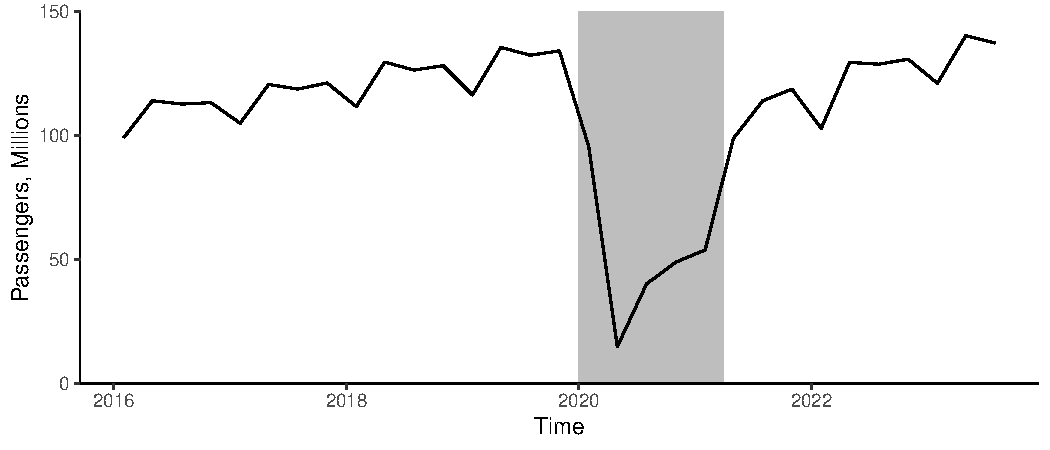
\includegraphics[width = \linewidth]{Quarterly_DB1B_Itineraries}
	\footnotesize{Source: DB1B Data. Shaded region depicts the duration of the coronavirus pandemic before widespread vaccine availability within the United States, namely, from the first quarter of 2020 through the first quarter of 2021.}
\end{figure}
    
	However, this recovery in ridership did not mark a return to the prior market conditions for the industry. Historically, approximately a third of air travel is motivated by business \citep{berry_tracing_2010, bet_market_2021}). However, following the pandemic, business travel decreased as businesses switched to telecommunications for meetings rather than face-to-face interactions \citep{semuels_business_2021}. Meanwhile, leisure travelers built savings during the decline in travel, allowing them to behave less price-sensitively following the pandemic. As such, the overall change in price elasticity is apriori ambiguous.\footnote{In a recent working paper, \citet{ewen_zoom_2023}, this phenomenon appears to have occurred, with a non-negligible share of leisure travelers being less price-sensitively than before the pandemic. In Table \ref{tab:DemandEst}, I find evidence that the demand for airfare has become slightly less elastic following the pandemic, consistent with the idea that this change in consumer behavior was enough to offset the changes from business travel on elasticity.}  As such, consumption patterns are liable to differ between the pre-pandemic and post-pandemic periods despite the large recovery in passenger levels. 

    
	\subsection{Attempted JetBlue-Spirit Merger}
	\label{sec:Setting_Merger}
	In February 2022, Spirit announced its intention to merge with fellow ultra-low cost carrier Frontier \citep{schaper_frontier-spirit_2022}. This prompted a counteroffer from JetBlue in April for ownership of Spirit, which would lead to the attempted merger between Spirit and Frontier being called off in July amid a lack of support from Spirit shareholders \citep{josephs_jetblue_2022, josephs_spirit_2022}. By mid-October, Spirit shareholders approved the acquisition by JetBlue \citep{koenig_spirit_2022}. The next year would see the United States Department of Justice, the District of Columbia, Massachusetts, and New York Attorneys General file suit to block the merger in March \citep{chokshi_justice_2023}. Following a trial in the winter of 2023, the merger would be blocked on January 16, 2024, and the parties would ultimately decide against appealing the verdict \citep{chapman_jetblue_2024}.  These events are summarized in Table \ref{tab:JetBlue_Spirit_Timeline}. 

    	\begin{table}[tb]
		\caption{JetBlue-Spirit Merger Timeline}
		\label{tab:JetBlue_Spirit_Timeline}
		\begin{center}
			\begin{tabular}{ccc}
				\hline
				Year & Date & Event \\
				\hline
				2022 & February 7 & Frontier-Spirit Merger Announced \\
				& April 5 &  First JetBlue Offer for Spirit Released\\
				& May 6 & Spirit Rejects JetBlue Offer \\
				& July 27 &  Frontier-Spirit Merger Attempt Collapses\\
				& July 28 &  Spirit Board Approves JetBlue Merger\\
				& October 19 & Spirit Shareholders Approve Merger \\
				\hline
				2023 & March 7 &  Department of Justice Files Suit\\
				& October 31 - December 5 &  JetBlue-Spirit Merger Trial \\
				\hline
				2024 & January 16 & JetBlue-Spirit Merger Blocked \\
				& March 4 & JetBlue, Spirit Drop Appeal Plans \\
			\end{tabular}
		\end{center}
	\end{table}

	JetBlue publicly considered the acquisition of Spirit to be a top priority for the company, choosing to not appeal the ruling blocking its Northeast Alliance with American Airlines in favor of focusing its resources on overcoming the lawsuit seeking to block the merger with Spirit \citep{aratani_jetblue_2023}. Beyond these legal resources, it directed resources toward trying to win public favor over the merger. Notably, it coordinated comment submissions to a Department of Transportation regulatory filing regarding the merger with pro-merger comments sourced from its employees.\footnote{Some employees went on to dispute that these comments accurately reflected their views \citep{birnbaum_elizabeth_2023, birnbaum_jet-blue_2023}. In Appendix \ref{sec:NaturalLanguage}, I use stance detection techniques to analyze comments left on this filing in more detail.} Despite this, following the ruling against the merger it would ultimately choose to drop its appeals, with some financial analysts noting a significant deterioration of Spirit's financial stability between 2022 and 2024 \citep{sider_jetblue_2024}. 
	
	I now turn my attention to the ruling in the case \citep{william_g_young_findings_2024} which ultimately blocked the JetBlue-Spirit merger attempt. The judgment identifies five key cities for his ruling: Orlando, San Juan, Miami and Fort Lauderdale (termed ``South Florida"), New York City, and Boston. These cities were identified on the basis that the majority of passengers in markets with competition between JetBlue and Spirit departed from these cities. These largely align with the cities in which the two firms would have the largest share of departing passengers within 2022 (Table \ref{tab:KeyCities}). However, the cities indicated ignores the firms' role in multiple smaller markets within Puerto Rico, namely Ponce and Aguadilla, where the two firms comprise the vast majority of the market. 
	
	In section 2.F of the judgment, the potential effects of the merger are listed as decreased airline seats, increased market concentration, increased debt for JetBlue, and increased prices for consumers. Table \ref{tab:JetBlueSpirit_Fleet} documents the aircraft in JetBlue and Spirit's fleets in 2022. Both airlines predominantly fly aircraft manufactured by Airbus. JetBlue's fleet is slightly more varied than Spirit's as it uses five different versions of the Airbus A321 aircraft\footnote{Two of these configurations reflect solely different seat configurations. The other three configurations are on the Airbus A321neo, a revision of the earlier aircraft.} Should Spirit's Airbus A320 and Airbus A321 have been adjusted to the predominant seat configurations of JetBlue's aircraft, a total of 20 seats would be lost on each Airbus A320 and 69 seats would be lost on each Airbus A321, for a total of 4,799 seats lost. This would reflect a loss of approximately 13\% of the seats on Spirit's aircraft.\footnote{If instead, Spirit's Airbus A321 were adjusted to the 200 seat configuration rather than the 159 configuration, then this would be 3500 seats lost or a loss of approximately 9.9\% of Spirit's seat capacity.} These rough calculations closely track the estimate of an 11\% reduction in seats accepted by the trial court in its decision.\footnote{The court further estimated a decline in annual departures of over 6.1 million. As I neither possess data on flight schedules nor model flight schedules endogenously, I am unable to assess this claim.} 
    
    \begin{table}
        \begin{center}
            \caption{JetBlue, Spirit Fleet Composition - 2022}
            \label{tab:JetBlueSpirit_Fleet}
            \vspace{-10mm}
          
\begin{tabular}[t]{llrrr}
\toprule
Manufacturer & Model & Seats & Count & Total Seats\\
\midrule
\addlinespace[0.3em]
\multicolumn{5}{l}{\textbf{JetBlue}}\\
\hspace{1em}Airbus & A220 & 140 & 14 & 1960\\
\hspace{1em}Airbus & A320 & 150 & 11 & 1650\\
\hspace{1em}Airbus & A320 & 162 & 119 & 19278\\
\hspace{1em}Airbus & A321 & 159 & 35 & 5565\\
\hspace{1em}Airbus & A321 & 200 & 28 & 5600\\
\hspace{1em}Airbus & A321neo & 138 & 5 & 690\\
\hspace{1em}Airbus & A321neo & 160 & 2 & 320\\
\hspace{1em}Airbus & A321neo & 200 & 16 & 3200\\
\hspace{1em}Embraer & E190 & 100 & 55 & 5500\\
\addlinespace[0.3em]
\multicolumn{5}{l}{\textbf{Spirit}}\\
\hspace{1em}Airbus & A319 & 145 & 31 & 4495\\
\hspace{1em}Airbus & A320 & 182 & 133 & 24206\\
\hspace{1em}Airbus & A321 & 228 & 30 & 6840\\
\bottomrule
\end{tabular}

        \end{center}
        \footnotesize{Source: B-43 Inventory Data.}
    \end{table}

    This paper estimates the counterfactual increase in market concentration and increase in prices in Section \ref{sec:Analysis_Merger}. 

    	
	\subsection{Northeast Alliance}
	\label{sec:Setting_NEA}
	
	Prior to its attempted merger with Spirit, JetBlue entered into the Northeast Alliance (NEA) with American Airlines at the start of 2021. The NEA saw the two firms coordinate operations to behave as a single carrier for routes that touched upon airports serving the New York City and Boston markets. They jointly decided their network for these routes, and operated them intending for consumers to be indifferent between the two carriers, worked to minimize overlap in product offerings on these routes, and shared revenue from products within the agreement. The United States Department of Justice along with six states and the District of Columbia brought a lawsuit against the agreement in September 2021 alleging violations of the Sherman Antitrust Act. Following a 2022 trial, the agreement would be found to violate the Sherman Antitrust Act in May 2023 and it was subsequently unwound \citep{rennison_jetblue-american_2023, rains_what_2023}.\footnote{Table \ref{tab:NEA_Timeline} details a timeline of key events relating to the NEA. Notably, some landing slot leases between the two airlines related to the merger experienced a gradual reversion to their original owners.} With this timeline outlined, I will now briefly discuss how the NEA differs from traditional aviation alliances and the issues it posses for estimation of the counterfactual merger effects for the JetBlue-Spirit merger. 

    \begin{table}[tb]
		\caption{Northeast Alliance Timeline}
		\label{tab:NEA_Timeline}
		\begin{center}
			\begin{tabular}{ccc}
				\hline
				Year & Date & Event \\
				\hline
				2020 & Quarter 1-2 & JetBlue and American Negotiate Alliance \\ 
				& July 16 & Northeast Alliance Announced \\
				& July 22 & Alliance Agreement submitted to DOT \\
				\hline 
				2021 & January 10 & DOT Terminates Antitrust Review \\
				& February 24 & Codesharing Agreement Begins on {X} Routes \\
				& May 26 & Reciprocal Loyalty Earnings Begins \\
				& Early September & NEA Shuttle at JFK Opens \\
				& September 21 & DOJ Files Lawsuit Against NEA \\  
				\hline
				2022 & September 27 - November 18 & NEA-Trial \\
				\hline 
				2023 & May 19 & NEA Ruled Anti-Competitive \\
				& July 5 & JetBlue Drops Appeal Plans \\
				& July 21 & NEA Codesharing Ends \\
				& October 31 & JFK Shuttle Ceases Operation\\
				& October 31 & 12 Slot Leases to JetBlue Terminate \\
				\hline 
				2024 &  March 31  & 27 Slot Leases to JetBlue Terminate \\ 
				& March 31 & 1 Slot Lease to American Terminates \\
				& October 26 & Remaining NEA Slot Leases Terminate				 \end{tabular}
		\end{center}
	\end{table}

	Alliances between aviation firms are commonplace within consumer aviation. For example, Delta is part of the ``SkyTeam Alliance" and United is part of the ``Star Alliance." These alliances see firms operating code-sharing agreements between different carriers, in which airlines can sell seats on flights operated by other airlines, with the ticket being under the ticketing airlines' code.\footnote{This allows, for example, for passengers of the Canadian airline Westjet to book connecting flights into the United States by using Delta flights for the intranational legs of their trip.}  These agreements are primarily operated between carriers situated in different countries which allows for better access to foreign markets as airlines are not normally able to fly routes entirely situated within a single foreign country. Benefits to consumers include the earning of frequent flier miles across all stages of a journey, regardless of the operating carrier, easier handling of baggage, and easier bookings. Meanwhile, carriers benefit from being able to offer a wider variety of destinations than would otherwise be possible.
	
	Domestic aviation alliances are rare at present. Unlike alliances between domestic and foreign carriers, these agreements are generally unable to receive waivers from antitrust proceedings through the Department of Justice and as such face additional regulatory scrutiny. Traditionally, these domestic agreements only apply to markets without both firms and the alliance's members otherwise maintain separate routing decisions, operations, and planning. One example of a currently active domestic aviation alliance is the West Coast Alliance between American and Alaska Airlines.  
	
	Contrasting this traditional approach, the NEA was structured to act more similarly to a merger on affected routes. The two firms jointly scheduled flights within the selected cities, minimized overlap on routes operated by both firms\footnote{It is not clear how effective this was. As documented in Figure \ref{fig:NEA_Operating}, the levels of shared routes at each of the four impacted airports was within historically normal ranges.}, and coordinated operations at the airports impacted by the agreement.\footnote{One example of this coordination is a shuttle operated by the two airlines at JFK to allow customers to transfer between the terminals used by each airline without having to clear security on a connecting trip \citep{griff_riding_2021}.} Furthermore, as two of the impacted airports featured slot and gate controls\footnote{A slot-controlled airport is one in which airlines are assigned specified time slots by the FAA for departures and arrivals to allow for better coordination of runway usage in congested airports. These slots are set in advance of individual operation days and can be transferred between airlines as if they were property of the airline which holds them.}, the NEA saw these firms share slot permits and share gates at the affected airports. This would be found by the trial court to have increased barriers to entering the New York City air travel market by deterring these firms by selling off landing slots to other firms. 
    
    The NEA impacts the evaluation of the counterfactual effects of the JetBlue-Spirit merger through its effects on the product offerings of JetBlue. Through jointly optimizing its network structure with American Airlines, JetBlue operated flights in different markets than it otherwise would have. As my simulation of the JetBlue-Spirit merger treats product offerings as exogenous, my post-pandemic results should be understood as estimating the world where the merger took place while the NEA was still in effect. 

    Beyond the changes to market structures, the NEA results in products within my sample that are assigned to JetBlue despite being operated solely or jointly with American. The majority of the NEA's existence saw over thirty products a quarter that fits these characteristics within markets that Spirit competes in (Table \ref{tab:NEA_Codesharing_Table}. As such, the recovery of marginal costs for these products is liable to be incorrect.  

	\section{Data and Summary Statistics}
	\label{sec:Data}
	The primary dataset used in the creation of this paper is the Bureau of Transportation Statistics' Airline Origin and Destination Survey (DB1B). The DB1B is a 10\% sample of all domestic airline itineraries within the United States. It includes data on pricing, distance, carrier, and number of connecting flights. Within the literature examining the aviation industry, it has been the preferred data for domestic air travel for decades (e.g. \citet{ciliberto_market_2021, berry_tracing_2010, goolsbee_how_2008, peters_evaluating_2006}). The sample used for the analyses in this paper covers the years between 2017 and 2023.  

    Despite the breadth of its included information, the DB1B has one key limitation - fares consist solely of the base airfare. As such, it does not include airline fees (such as for checked bag fees) nor additional amenities purchased by consumers as part of their travel. As Spirit and the other ultra-low cost carriers focus on ``unbundled" fares, these airline fares are liable to be reported as systematically lower than the full price paid by consumers after taking into account spending on auxiliary purchases.\footnote{Legacy carriers have instituted a tier of fare known within the industry as ``basic economy" to compete with Spirit through a limited amount of unbundled fares. As such, these fares are likewise lower than the true amount paid by consumers. Unfortunately, the DB1B does not include reliable information on fare class, and as such, these fares are unable to be detected.} This inhibits a proper simulation of changes to consumer surplus following the merger, as discussed in more detail in Section \ref{sec:Analysis_Merger}. Within this section, I further detail how the use of minimum fare data may allow us to capture some understanding of the consumer surplus change of marginal travelers.  
    	
	Markets are defined by origin airport, destination airport, year, and quarter. Within this definition, originating and terminating airports are treated as the determinants of a market rather than airports' metropolitan statistical areas. Notably, the decision to define markets by airports or cities is divisive within the literature. It is known within the literature that consumers do not treat airports within a metropolitan statistical area as interchangeable.\footnote{\citet{goolsbee_how_2008}, for example, observes differential impacts on pricing of possible firm entry at the airport level than would be expected if airports within a metropolitan statistical area were treated as interchangeable by consumers.} Within this paper, products within a market are further defined by both ticketing carrier and non-stop status.\footnote{As such, each carrier can have zero, one, or two products within a market.} Appendix \ref{sec:DataProcessing} details the sample construction methodology and restrictions on markets and itineraries included within the sample (such as excluding markets that consist of airports that are fewer than 150 miles apart).
	
	Market size is defined as the geometric mean of the population of the origin and destination metropolitan statistical areas population. This is a standard assumption within this literature \citep{ciliberto_market_2021}. This is calculated using the United States Census Bureau's annual estimates of metropolitan statistical area population. The outside good within a market is defined as the decision not to consume air travel between an origin and destination airport pair. As such, the outside good includes not making a trip, making a trip by car or bus, and making a trip between two different airports within the same origin and destination metropolitan areas. 
    
    \begin{table}
    \caption{Product Level Summary Statistics}
    \label{tab:Summary_Statistics_Product}
                    \vspace{-15mm}
                    \begin{center}
    
\begin{tabular}[t]{llllll}
\toprule
 & Mean & (SD) & Minimum & Median & Maximum\\
\midrule
\addlinespace[0.3em]
\multicolumn{6}{l}{\textbf{Pre-Pandemic}}\\
\hspace{1em}Price (2017 USD) & 232.21 & ( 70.12 ) & 33.12 & 235.62 & 810.58\\
\hspace{1em}Passengers & 4248.33 & ( 10185.27 ) & 100 & 810 & 192050\\
\hspace{1em}Distance (1000s) & 1.41 & ( 0.67 ) & 0.15 & 1.28 & 3.87\\
\hspace{1em}Extra Distance & 0.13 & ( 0.18 ) & 0 & 0.06 & 1.66\\
\hspace{1em}Nonstop & 0.28 & ( 0.45 ) & 0 & 0 & 1\\
\hspace{1em}Origin Destinations & 29.97 & ( 33.37 ) & 1 & 13 & 180\\
\hspace{1em}Origin Prescence (\textbackslash{}\%) & 36.23 & ( 31.26 ) & 0.54 & 19.51 & 100\\
\hspace{1em}Delta & 0.25 & ( 0.43 ) & 0 & 0 & 1\\
\hspace{1em}American & 0.22 & ( 0.41 ) & 0 & 0 & \vphantom{1} 1\\
\hspace{1em}United & 0.14 & ( 0.35 ) & 0 & 0 & 1\\
\hspace{1em}Southwest & 0.25 & ( 0.43 ) & 0 & 0 & 1\\
\hspace{1em}JetBlue & 0.03 & ( 0.17 ) & 0 & 0 & 1\\
\hspace{1em}Spirit & 0.03 & ( 0.18 ) & 0 & 0 & 1\\
\hspace{1em}Other Carrier & 0 & ( 0.06 ) & 0 & 0 & 1\\
\hspace{1em}Observations & 307849 &  &  &  & \\
\addlinespace[0.3em]
\multicolumn{6}{l}{\textbf{Post-Pandemic}}\\
\hspace{1em}Price (2017 USD) & 212.77 & ( 75.21 ) & 27.96 & 209.94 & 737.78\\
\hspace{1em}Passengers & 3531.43 & ( 8648.27 ) & 100 & 690 & 144930\\
\hspace{1em}Distance (1000s) & 1.41 & ( 0.67 ) & 0.15 & 1.28 & 3.86\\
\hspace{1em}Extra Distance & 0.14 & ( 0.19 ) & 0 & 0.07 & 1.83\\
\hspace{1em}Nonstop & 0.26 & ( 0.44 ) & 0 & 0 & 1\\
\hspace{1em}Origin Destinations & 29.24 & ( 33.72 ) & 1 & 12 & 187\\
\hspace{1em}Origin Prescence (\textbackslash{}\%) & 34.77 & ( 30.92 ) & 0.53 & 18.42 & 100\\
\hspace{1em}Delta & 0.22 & ( 0.41 ) & 0 & 0 & 1\\
\hspace{1em}American & 0.22 & ( 0.41 ) & 0 & 0 & 1\\
\hspace{1em}United & 0.13 & ( 0.34 ) & 0 & 0 & 1\\
\hspace{1em}Southwest & 0.26 & ( 0.44 ) & 0 & 0 & 1\\
\hspace{1em}JetBlue & 0.03 & ( 0.16 ) & 0 & 0 & 1\\
\hspace{1em}Spirit & 0.04 & ( 0.2 ) & 0 & 0 & 1\\
\hspace{1em}Other Carrier & 0.01 & ( 0.1 ) & 0 & 0 & 1\\
\hspace{1em}Observations & 265196 &  &  &  & \\
\bottomrule
\end{tabular}

                        \end{center}
                    \vspace{-5mm}
    \footnotesize{A product is defined as a set of origin airport, destination airport, year, quarter, firm, and nonstop status. ``Origin Destinations" is the number of airports served from the originating airport across all firms, ``Origin Prescence" is the fraction of these destinations served by the ticketing carrier. The pre-pandemic sample includes all quarters of the years 2017 through 2019. The post-pandemic sample includes data from the second quarter of 2021 through the second quarter of 2023. The 'Other' carrier contains the products of minor carriers that operate within the industry, such as Sun Country. Alaska Airlines, Allegiant Air, and Frontier Airlines are not classified as this.}
    \end{table}

    Summary statistics for product-level data are included in Table \ref{tab:Summary_Statistics_Product}. Both product prices and passengers fell on average following the pandemic, with the average itinerary becoming \$22 cheaper in real terms while having 700 fewer passengers. Notably, despite the post-pandemic period's economy having high levels of inflation, there is only a \$6 increase in nominal average fares between the two periods.  Delta's representation in the observed products slightly decreased by 3 percentage points while Southwest, Spirit, and the `Other' carrier\footnote{The 'Other' carrier contains the products of minor carriers that operate within the industry, such as Sun Country. Alaska Airlines, Allegiant Air, and Frontier Airlines are not classified as this.} increased their product offerings by approximately one percentage point. As such, products are broadly similar between the two periods in terms of their operating carriers. Finally, products are slightly less likely to include an intermediate stop following the pandemic and cover slightly smaller distances. 

    Summary statistics for market-level characteristics are included in Table \ref{tab:Summary_Statistics_Market}. Despite the post-pandemic period having fewer overall markets included in the sample due to spanning a smaller period of time, JetBlue and Spirit competed in over a hundred additional markets in this period than in the three years before the pandemic. Additionally, there was on average roughly a third of an additional firm in the post-pandemic period in the average market, driven by firms operating a single product within the market. Finally, it is worth noting that the number of customers within the average market decreased by approximately 16,000 customers between the two periods. Aside from this, overall market characteristics are similar in terms of miles flown between the two periods. 

    \begin{table}
        \caption{Market Level Summary Statistics}
        \label{tab:Summary_Statistics_Market}
                \vspace{-15mm}
\begin{center}
            
\begin{tabular}[t]{llllll}
\toprule
 & Mean & (SD) & Minimum & Median & Maximum\\
\midrule
\addlinespace[0.3em]
\multicolumn{6}{l}{\textbf{Pre-Pandemic}}\\
\hspace{1em}Minimum Miles (1000s) & 1.18 & (0.64) & 0.15 & 1.02 & 2.95\\
\hspace{1em}Average Miles (1000s) & 1.23 & (0.66) & 0.15 & 1.07 & 3.02\\
\hspace{1em}Number of Firms & 2.94 & (1.49) & 1 & 3 & 9\\
\hspace{1em}Number of Products & 3.52 & (2.11) & 1 & 3 & 15\\
\hspace{1em}Number of Customers & 14970.24 & (28280.06) & 260 & 4150 & 406050\\
\hspace{1em}HHI & 8017.21 & (4297.27) & 1611.61 & 7043.02 & 20000\\
\midrule
\hspace{1em}Observations & 87363 &  & JetBlue Markets & 7442 & \\
\hspace{1em}JetBlue \& Spirit Markets & 1533 &  & Spirit Markets & 7474 & \\
\midrule
\addlinespace[0.3em]
\multicolumn{6}{l}{\textbf{Post-Pandemic}}\\
\hspace{1em}Minimum Miles (1000s) & 1.19 & (0.64) & 0.15 & 1.04 & 2.96\\
\hspace{1em}Average Miles (1000s) & 1.24 & (0.66) & 0.15 & 1.1 & 2.98\\
\hspace{1em}Number of Firms & 3.21 & (1.56) & 1 & 3 & 9\\
\hspace{1em}Number of Products & 3.79 & (2.16) & 1 & 3 & 14\\
\hspace{1em}Number of Customers & 13375.81 & (25085.61) & 230 & 3840 & 317370\\
\hspace{1em}HHI & 7479.76 & (4410.86) & 1460.46 & 6260.03 & 20000\\
\midrule
\hspace{1em}Observations & 70016 &  & JetBlue Markets & 5945 & \\
\hspace{1em}JetBlue \& Spirit Markets & 1554 &  & Spirit Markets & 9123 & \\
\bottomrule
\end{tabular}

            \end{center}
    \vspace{-5mm}
            \footnotesize{A market is defined as a combination of origin airport, destination airport, year, and quarter. The average miles reported within a market is weighted by itinerary passengers. The pre-pandemic sample includes all quarters of the years 2017 through 2019. The post-pandemic sample includes data from the second quarter of 2021 through the second quarter of 2023. JetBlue (Spirit) markets is the total number of markets operated by JetBlue (Spirit) within the period of observation. ``JetBlue \& Spirit Markets" is the total number of markets with both firms competing within them.}

    \end{table}

	\section{Analysis}
	\label{sec:Analysis} 	 
 	 	 
	\subsection{Demand}
	\label{sec:Analysis_Demand}
	I use a random coefficient nested logit model to estimate demand. Within the industrial organization literature focused on airlines, practitioners generally estimate demand through the application of either the nested logit model (such as in \citet{turner_access_2022,ciliberto_market_2021, aguirregabiria_dynamic_2012}) or the random coefficient logit model originally described in \citet{berry_automobile_1995}.\footnote{\citet{bet_market_2021} is an example of existing literature which uses the random coefficient nested logit model.} Examples of the use of the nested logit model include   \citet{turner_access_2022,ciliberto_market_2021, aguirregabiria_dynamic_2012}; examples of the use of the random coefficient logit model include \citet{ gayle_efficiency_2013, berry_tracing_2010}. Through the use of random coefficients and a nested logit structure for the random errors, the random coefficient nested logit model is able to better approximate own-price and cross-price elasticities than the other models, at the cost of increased computational requirements \citep{grigolon_nested_2014}. That the random coefficient nested logit estimates each type of price elasticity more reliable than the other models is of particular importance to this work as those are core inputs used for the estimation of marginal costs and shares within the merger simulation detailed in Section \ref{sec:Analysis_Merger}. 
    
    Adopting the notation described in \citet{conlon_best_2020}, each consumer $i$ in market $t$ has indirect utility from buying product $j$ as defined by 
	
	\[U_{ijt} = \delta_{jt} + \mu_{ijt} + \epsilon_{ijt}\] where $\delta_{jt}$ is the mean utility across consumers in market $t$ for product $j$, $\mu_{ijt}$ is each consumer's deviation from this mean utility, and $\epsilon_{ijt}$ is an unobserved consumer-level shock. The mean utility across consumers $\delta_{jt}$ is parameterized as \[\delta_{jt} = \alpha p_{jt} + x_{j} \beta + F_{jt}\gamma  +  \zeta_{jt}\] where $p_{jt}$ is the price of product $j$ in market $t$; $x_{jt}$ is a vector of observed itinerary characteristics including nonstop flight status, miles flown, the square of the miles flown, the percent of destinations from the originating airport served by the airline, the extra miles traveled\footnote{This is defined as being the difference between each product's miles traveled and the minimum miles traveled within the market.}, the square of the extra miles traveled, and a dummy variable which is 1 if the route serves a market including either an end point in Las Vegas or a market in the state of Florida; $F_{jt}$ is a vector of carrier and time fixed effects; and $\zeta_{jt}$ is a product level shock shared by all consumers within a market.\footnote{This includes characteristics of products unobserved by the author, such as advertising.} The non-price product characteristics included here are intended to be largely unresponsive to demand shocks - these characteristics of a product are determined primarily by a carrier's network structure and the geography between the origin and destination airports. As such, these characteristics should not change in response to unobserved quarterly demand shocks.
	 
    Finally, the consumer specific deviation from utility, $\mu_{ijt}$, is parameterized as \[\mu_{ijt} = \sigma_{p} p_{jt} \nu_{ip} + \sigma_{n} n_{jt} \nu_{in} + \sigma_{m} m_{jt} \nu_{im} \] with the $\nu$ parameters drawn from a standard normal distribution, $p$ the product's price, $n$ the product's nonstop status, and $m$ the miles flown for the product. Each parameter $\sigma$ within this model represents the standard deviation of consumers preferences for this product.  Finally, $\epsilon_{ijt}$ are assumed to arise from a type 1 extreme value distribution so that market shares will be of the discrete choice nested logit variety. Within this model specification, air travel is included within one nest while the outside good\footnote{Which both includes the decision to not travel within the market or to travel by other means, such as train or car.} is included in the other nest. Utility of the outside good is normalized to zero. 
	
	Consumer $i$ purchases itinerary $j$ if it has greater utility than all other products in the market. As such, market shares can be obtained by integrating over the consumers within the market, resulting in the market share of each product being defined by \[s_{jt} = \int \frac{e^{\delta_{jt} + \mu_{ijt}}}{\sum_{j'} e^{\delta_{jt} + \mu_{ijt}}} d{\nu_{i}}\]
	
	 Four sets of instruments are used to account for the endogeneity of prices and shares within a market. The first set consists of a dummy variable which is 1 if at least one of the endpoint airports is a hub of the ticketing carrier, the product of this variable with the miles traveled, and the product of this with the square of the miles traveled. These serve as cost shifters.\footnote{In constructing the data, a round-trip fare is divided into two unidirectional fares each with imputed fare equal to half of the overall payment made. This motivates the symmetric treatment of both origin hubs and destination hubs in the construction of these instruments.} The second set of instruments, employed to account for endogeneity of market shares, consists of the differentiation instruments described in \citet{gandhi_measuring_2019} constructed from a dummy variable for nonstop flight status, the distance traveled, the square of the distance, and the service ratio of the ticketing carrier out of the destination airport. The third set of instruments, employed to instrument for the nesting parameter $\lambda$ consists solely of the number of products within a market to assist in model convergence. Finally, all remaining exogenous regressors and their interactions comprise the final set of instruments.\footnote{Other instruments for price were considered, including interactions between the gas miles variable and characteristics of the origin airport and interactions between the exogenous variables. However, the selection of price shifters used in the final model had the best performance across the tests documented in Tables \ref{tab:Instrument_Compare_Pre}. The final specification chosen (column 4) has the benefit of passing the Wu-Hausman test while failing the Test of Over Identification by the least amount of the tested models. As noted in \citet{nevo_measuring_2001}, provided enough observations it is virtually impossible to pass this, and as such, I am not concerned with the result. For comparison purposes, the instrument comparison table on the post-pandemic period (2021 Q2 through 2023 Q2) is included as Table \ref{tab:PostPand_Instrument_Compare}.}
	
    Results for the estimation of this model's coefficients for both periods are included in Table \ref{tab:DemandEst}. With the exception of nonstop flight status and the tourist route dummy variable, all variables are predicted to influence consumer demand in both periods. That the estimated coefficient on nonstop flight status is insignificant is not concerning as the model additionally includes variables which measure the responsiveness of consumers to extra miles traveled over the minimum in the market, which were strongly significant. As such, consumer behavior in regard to nonstop flights is not different than would be expected.  
    
    Of the variables which allow for random effects, only price takes a significant coefficient, of roughly $0.6$. Finally, I estimate a nesting parameter of a little over a tenth in both periods. This is consistent with high degrees of substitutability between air travel and the outside good, which is inconsistent with most previous literature's estimates of the nesting parameter for similar models. As such, consumers are predicted to have a high willingness to enter (leave) the market in response to a price decrease (increase).

     JetBlue's products face more elastic demand than Spirit's, consistent with the firm targeting less budget conscious travelers than Spirit. Consumer preferences are estimated to have become less price elastic between the pre-pandemic and post-pandemic periods. This suggests that despite the decline in business travel following the pandemic, leisure travelers' spending patterns changed to be less price sensitive, perhaps due to excess savings acquired during the pandemic period or the desire to makeup for lost vacations.\footnote{A working paper, \citet{ewen_zoom_2023}, which uses structural modeling on data from 2019 and 2022 observes similar patterns.}  The estimated coefficient on tourist routes is consistent with this change in consumption patterns.  It is strongly significant in the post-pandemic period but not the pre-pandemic period, consistent with the notion of increased tourism levels. 
    
    \begin{table}
        \caption{Demand Estimation Results}
        \label{tab:DemandEst}
        \vspace{-15mm}
        \begin{center}
        
\begin{tabular}[t]{lll}
\toprule
Variable & Post-Pandemic & Pre-Pandemic\\
\midrule
Price & -3.114 & -2.947\\
 & (0.44) & (0.34)\\
\midrule
Price & 0.599 & 0.59\\
 & (0.12) & (0.12)\\
\midrule
Nesting Parameter & 0.115 & 0.136\\
\addlinespace
 & (0.032) & (0.045)\\
\midrule
Period & 2017Q1-2019Q4 & 2021Q2-2023Q2\\
N Products & 265196 & 307849\\
N Markets & 70016 & 87363\\
Mean Elasticity & -5.211 & -5.323\\
\addlinespace
Spirit Mean Elasticity & -3.44 & -3.15\\
JetBlue Mean Elasticity & -5.18 & -5.16\\
Mean Markup & 0.21 & 0.203\\
\bottomrule
\end{tabular}
   
        \end{center}
        \vspace{-5mm}
                \footnotesize{$^{***}p<0.01$; $^{**}p<0.05$; $^{*}p<0.1$ Products are defined as a Carrier-Nonstop pair within an Origin-Destination-Year-Quarter market. Origin Service Ratio is the fraction of direct routes out of the originating airport operated by the carrier divided by the number of distinct direct routes out fo that airport. Extra Miles is the average additional miles flown with a connecting itinerary minus the minimum miles flown within a market.  A tourist product is one that serves the Las Vegas metropolitan statistical area or an airport in Florida.}

    \end{table}
		
	\subsection{Supply}
	\label{sec:Analysis_Supply}
	I assume that each aviation market is assumed to operate under Bertrand competition with differentiated products following the exogenous determination of quarterly route structure. As derived in \citet{berry_automobile_1995}, under this assumed market structure, profit maximizing firms will choose prices such that \[P = MC + \Delta^{-1} s\] where $MC$ is marginal cost and $\Delta = - \mathcal{H} \cdot \frac{\partial s}{\partial p}^{'}$.\footnote{To ease readability, I adopt the notation of \citet{conlon_best_2020}.} $\mathcal{H}$ is an ownership matrix; within $\mathcal{H}$, $\mathcal{H}_{i,j} = 1$ if the same firm produces both products $i$ and $j$ and is zero otherwise.

    Through the pricing condition and the estimated own-price and cross-price elasticities, I am able to estimate both marginal costs and markups. Information on the distribution of these are included with the estimates of demand within Table \ref{tab:DemandEst}. I estimate a slight increase in markups of approximately two percentage points between the pre- and post-pandemic periods. 
	
	
	\subsection{Merger Simulation}
	\label{sec:Analysis_Merger}
	With the demand and supply models used within this paper described, I can now turn my attention to the simulation of the JetBlue-Spirit merger. For each of the pre-pandemic and post-pandemic periods, I estimate three counterfactual situations. These are respectively, a best case merger (where the merged product takes the lowest marginal cost and best unobservables of the two products), an average case merger (where the merged product takes the average of the two firms marginal costs and the average of the estimated unobservables), and a worst case scenario (where the merged product takes the greater of the marginal costs of the two firms and the lowest estimated unobservable characteristics).\footnote{The choice of these as the simulation specifications has its roots in \citet{ciliberto_market_2021} which observes that the use of these specifications allows for analysis of the robustness of the results to different assumptions on how the merged firms products are realized. Beyond \citet{ciliberto_market_2021}, the use of multiple merger specifications, generally including a `best case' merger specification for consumer welfare is common within this literature (e.g. \citet{li_repositioning_2022}).} In each of these scenarios, I assume that the combined firm's connecting products take on the minimum of the miles flown, implicitly assuming that in all of these simulations that the combined firm will take advantage of better routing.\footnote{Furthermore, all products of the combined firm are coded as being operated by JetBlue for the purposes of carrier fixed effects.} Two alternative specifications for these simulations, where the merged firm's marginal costs decrease by either 5\% or 10\% are reported in Appendix \ref{App:Efficiencies}. The results for these alternative specifications are broadly consistent with the results discussed within this section.

    % Detail how this works mathematically
     
	 Table \ref{tab:Simulation_Price} contains the estimated price effects from the merger on individual product prices for markets that both firms competed in. In the best case scenario, I consistently estimate declines in the average prices of products in markets wherein both JetBlue and Spirit competed of between 13\% and 15\%, or approximately \$23 and \$29, regardless of sample period. In the worst case scenario, I estimate a minimal increase in average market fares for the pre-pandemic period and an increase of approximately 5\% in the post-pandemic period. 
     
    \begin{table}
        \caption{Simulated Price Effects of Merger - Joint Markets}
        \label{tab:Simulation_Price}
                \vspace{-15mm}
        \begin{center}
         
\begin{tabular}[t]{lllllll}
\toprule
 & N & Mean & (SD) & Minimum & Median & Maximum\\
\midrule
\addlinespace[0.3em]
\multicolumn{7}{l}{\textbf{Pre-Pandemic}}\\
\addlinespace[0.3em]
\multicolumn{7}{l}{\textbf{Product Prices (100s, 2017 USD)}}\\
\hspace{1em}\hspace{1em}Observed & 12074 & 2.04 & (0.69) & 0.47 & 1.98 & 4.91\\
\hspace{1em}\hspace{1em}Best Case & 10106 & 2.08 & (0.66) & 0.46 & 2.02 & 5.08\\
\hspace{1em}\hspace{1em}Average Case & 10106 & 2.12 & (0.64) & 0.46 & 2.06 & 5.14\\
\hspace{1em}\hspace{1em}Worst Case & 10106 & 2.16 & (0.64) & 0.48 & 2.09 & 5.13\\
\addlinespace[0.3em]
\multicolumn{7}{l}{\textbf{Market Average Price}}\\
\hspace{1em}\hspace{1em}Observed & 1418 & 2.01 & (0.43) & 0.93 & 1.95 & \vphantom{1} 3.1\\
\hspace{1em}\hspace{1em}Best Case & 1418 & 1.73 & (0.6) & 0.81 & 1.55 & \vphantom{1} 3.44\\
\hspace{1em}\hspace{1em}Average Case & 1418 & 2 & (0.51) & 1.01 & 1.92 & \vphantom{1} 3.38\\
\hspace{1em}\hspace{1em}Worst Case & 1418 & 2.01 & (0.5) & 1 & 1.92 & \vphantom{1} 3.5\\
\addlinespace[0.3em]
\multicolumn{7}{l}{\textbf{\% Change Average Price}}\\
\hspace{1em}\hspace{1em}Best Case & 1418 & -15.13 & (16.83) & -53.06 & -16.77 & 31.42\\
\hspace{1em}\hspace{1em}Average Case & 1418 & -0.7 & (10.36) & -38.87 & -0.19 & 39.57\\
\hspace{1em}\hspace{1em}Worst Case & 1418 & 0.18 & (10.27) & -34.26 & 0.61 & 37.41\\
\addlinespace[0.3em]
\multicolumn{7}{l}{\textbf{Median Price}}\\
\hspace{1em}\hspace{1em}Observed & 1418 & 2.01 & (0.43) & 0.93 & 1.95 & 3.1\\
\hspace{1em}\hspace{1em}Best Case & 1418 & 1.73 & (0.6) & 0.81 & 1.55 & 3.44\\
\hspace{1em}\hspace{1em}Average Case & 1418 & 2 & (0.51) & 1.01 & 1.92 & 3.38\\
\hspace{1em}\hspace{1em}Worst Case & 1418 & 2.01 & (0.5) & 1 & 1.92 & 3.5\\
\midrule
\addlinespace[0.3em]
\multicolumn{7}{l}{\textbf{Post-Pandemic}}\\
\addlinespace[0.3em]
\multicolumn{7}{l}{\textbf{Product Prices  (100s, 2017 USD)}}\\
\hspace{1em}\hspace{1em}Observed & 13650 & 1.96 & (0.78) & 0.35 & 1.89 & 5.25\\
\hspace{1em}\hspace{1em}Best Case & 11496 & 2.01 & (0.77) & 0.4 & 1.94 & 5.34\\
\hspace{1em}\hspace{1em}Average Case & 11496 & 2.05 & (0.74) & 0.4 & 1.99 & 5.33\\
\hspace{1em}\hspace{1em}Worst Case & 11496 & 2.1 & (0.74) & 0.41 & 2.04 & 5.33\\
\addlinespace[0.3em]
\multicolumn{7}{l}{\textbf{Market Average Price}}\\
\hspace{1em}\hspace{1em}Observed & 1554 & 1.95 & (0.55) & 0.65 & 1.89 & \vphantom{1} 3.57\\
\hspace{1em}\hspace{1em}Best Case & 1554 & 1.71 & (0.68) & 0.61 & 1.68 & \vphantom{1} 3.67\\
\hspace{1em}\hspace{1em}Average Case & 1554 & 2.04 & (0.64) & 0.76 & 1.95 & \vphantom{1} 3.85\\
\hspace{1em}Worst Case & 1554 & 2.06 & (0.64) & 0.76 & 1.96 & \vphantom{1} 3.93\\
\addlinespace[0.3em]
\multicolumn{7}{l}{\textbf{\% Change Average Price}}\\
\hspace{1em}Best Case & 1554 & -13.67 & (18.18) & -59.32 & -10.99 & 39.39\\
\hspace{1em}Average Case & 1554 & 4.21 & (9.96) & -32.12 & 4.07 & 49.1\\
\hspace{1em}Worst Case & 1554 & 5.38 & (10) & -33.29 & 5.03 & 50.4\\
\addlinespace[0.3em]
\multicolumn{7}{l}{\textbf{Median Price}}\\
\hspace{1em}Observed & 1554 & 1.95 & (0.55) & 0.65 & 1.89 & 3.57\\
\hspace{1em}Best Case & 1554 & 1.71 & (0.68) & 0.61 & 1.68 & 3.67\\
\hspace{1em}Average Case & 1554 & 2.04 & (0.64) & 0.76 & 1.95 & 3.85\\
\hspace{1em}Worst Case & 1554 & 2.06 & (0.64) & 0.76 & 1.96 & 3.93\\
\bottomrule
\end{tabular}

        \end{center}
        \vspace{-5mm}
        \footnotesize{Products from markets without both JetBlue and Spirit present are excluded. Distribution of changes of average market fares are graphed in Figures \ref{fig:AverageFare_ChangeDist_PrePandemic} and \ref{fig:AverageFare_ChangeDist_PostPandemic} for the pre-pandemic and post-pandemic periods respectively.}

     \end{table}

    Notably, JetBlue was clear on its intention to retire the Spirit business model following the acquisition and retool all Spirit aircraft to follow the JetBlue configuration. As such, it is worthwhile to examine changes in estimated pricing and costs on market fares in markets in which Spirit competed but not JetBlue. In reality, prices would change in these markets due to the retirement of the Spirit brand and adjustment to the higher cost JetBlue model. However, as I do not have estimates of marginal costs for the JetBlue operational model for these markets, we will instead solely focus on the changes due to the change from Spirit to JetBlue brand which would underestimate the true price changes. The results of this simulation are described in Table \ref{tab:Simulation_Price_Spirit}.\footnote{As the different simulations are defined by the method used to combine products between the two firms, all simulations are equivalent for markets with only Spirit within them.} Within these markets, I estimate that the average market would experience an increase in average fare of approximately 3.4\% in the pre-pandemic period and 9.7\% in the post-pandemic period. This finding reflects the negative consumer valuation of Spirit products over JetBlue products within the estimated demand models.

    \begin{table}
        \caption{Simulated Price Effects of Merger - Spirit Markets}
        \label{tab:Simulation_Price_Spirit}
                        \vspace{-15mm}
        \begin{center}
              
\begin{tabular}[t]{lllllll}
\toprule
 & N & Mean & (SD) & Minimum & Median & Maximum\\
\midrule
\addlinespace[0.3em]
\multicolumn{7}{l}{\textbf{Pre-Pandemic}}\\
\addlinespace[0.3em]
\multicolumn{7}{l}{\textbf{Prices (100s, 2017 USD)}}\\
\hspace{1em}\hspace{1em}Observed & 37776 & 2.1 & (0.78) & 0.38 & 2.08 & 7.17\\
\hspace{1em}\hspace{1em}Simulated & 30012 & 2.23 & (0.7) & 0.38 & 2.23 & 7.27\\
\addlinespace[0.3em]
\multicolumn{7}{l}{\textbf{Market Average Price}}\\
\hspace{1em}\hspace{1em}Observed & 5735 & 2.08 & (0.46) & 0.7 & 2.08 & 4.61\\
\hspace{1em}\hspace{1em}Simulated & 5735 & 2.14 & (0.55) & 0.59 & 2.13 & 4.75\\
\addlinespace[0.3em]
\multicolumn{7}{l}{\textbf{\% Change Average Price}}\\
\hspace{1em}\hspace{1em}Simulated & 5735 & 3.41 & (15.12) & -56.96 & 3.01 & 88.36\\
\addlinespace[0.3em]
\multicolumn{7}{l}{\textbf{Post-Pandemic}}\\
\addlinespace[0.3em]
\multicolumn{7}{l}{\textbf{Prices  (100s, 2017 USD)}}\\
\hspace{1em}\hspace{1em}Observed & 49630 & 1.97 & (0.82) & 0.29 & 1.95 & 6.27\\
\midrule
\hspace{1em}\hspace{1em}Simulated & 40330 & 2.17 & (0.77) & 0.32 & 2.17 & 6.88\\
\addlinespace[0.3em]
\multicolumn{7}{l}{\textbf{Market Average Price}}\\
\hspace{1em}\hspace{1em}Observed & 7569 & 1.97 & (0.53) & 0.6 & 1.94 & 4.07\\
\hspace{1em}\hspace{1em}Simulated & 7569 & 2.16 & (0.62) & 0.72 & 2.13 & 5.52\\
\addlinespace[0.3em]
\multicolumn{7}{l}{\textbf{\% Change Average Price}}\\
\hspace{1em}\hspace{1em}Simulated & 7569 & 9.71 & (12.21) & -44.52 & 9.65 & 75.68\\
\bottomrule
\end{tabular}

        \end{center}
        \vspace{-5mm}
        \footnotesize{Products are solely those from markets in which Spirit operated but not JetBlue.}
    \end{table}

     % Heterogeneity

     Now, I turn my attention to consumer welfare. Unfortunately, calculating consumer surplus is impossible with the available data from the DB1B. As alluded to in Section \ref{sec:Data}, Spirit offers "unbundled" fares which have additional fees required for the various amenities included in the base price of tickets for other firms (such as carry-on baggage). Consumers who would pay these fees at Spirit would have their change in consumer welfare overestimated traditional consumer surplus estimation techniques. Furthermore, as these fees differ between both customers and markets due to the use of algorithmic pricing \citep{senate_permanent_committee_on_investigations_majority_2024} it is unfortunately infeasible to do back-of-the-envelope estimations to try to recover the ``true," fee-inclusive, Spirit fares. 
     
     This motivates the consideration of another measure of consumer welfare, namely, the minimum fare available within each market. As noted by Judge Young in the merger trial, a large component of Spirit's customer base was highly price sensitive travelers who may not have been able to fly without the smaller base fares provided by Spirit. As such, it stands to reason that minimum fares within markets, in addition to the average fares, are important for understanding the counterfactual effects of the merger. 
     
     The overall change in minimum market fares, in twenty dollar intervals, is detailed in Table \ref{tab:MinimumPrice}. Across the simulations of price changes within markets that both firms competed in, at least 35 (of the 1418 (1554) markets that both firms competed in within the pre-pandemic (post-pandemic) period), markets in each period are estimated to have the minimum price within the market increase by over \$60. Within both periods, these markets are primarily between airports in the New York and Boston areas and various destinations within the Southern portion of the United States (such as Houston and Dallas). As such, it is consistent with the finding of the key markets of concern within the trial. 

    \begin{table}
        \caption{Change in Minimum Fare Available in Market (2017 USD)}
        \label{tab:MinimumPrice}
                \vspace{-15mm}
        \begin{center}
            
\begin{tabular}[t]{lrrrrrr}
\toprule
\multicolumn{1}{c}{ } & \multicolumn{3}{c}{Pre-Pandemic} & \multicolumn{3}{c}{Post-Pandemic} \\
\cmidrule(l{3pt}r{3pt}){2-4} \cmidrule(l{3pt}r{3pt}){5-7}
 & Best & Average & Worst & Best & Average & Worst\\
\midrule
$<$ 0 & 256 & 202 & 158 & 376 & 302 & 235\\
0-20 & 1151 & 612 & 539 & 1050 & 546 & 526\\
20-40 & 62 & 475 & 330 & 56 & 387 & 261\\
40-60 & 33 & 180 & 296 & 36 & 214 & 249\\
60-80 & 20 & 48 & 168 & 25 & 79 & 181\\
80 $<$ & 11 & 16 & 42 & 11 & 26 & 102\\
\bottomrule
\end{tabular}

        \end{center}
        \vspace{-5mm}
        \footnotesize{Products from markets without both JetBlue and Spirit present are excluded. The best case merger scenario is one in which the combined firm inherits the minimum average cost and greatest unobservables of each firm, the average case merger scenario has the combined JetBlue-Spirit inherit the average of the two firms' product characteristics, and the worst case scenario has the combined JetBlue-Spirit inherit the greatest marginal cost and lowest unobserveables. Prices are in 2017 dollars. A version of this table which reports the change in minimum fares in percent terms is included as Table        \ref{tab:MinimumPrice_Percent}.}
    \end{table}    

      \begin{figure}
    \caption{Simulated Change in Pre-Pandemic Minimum Market Fares}
    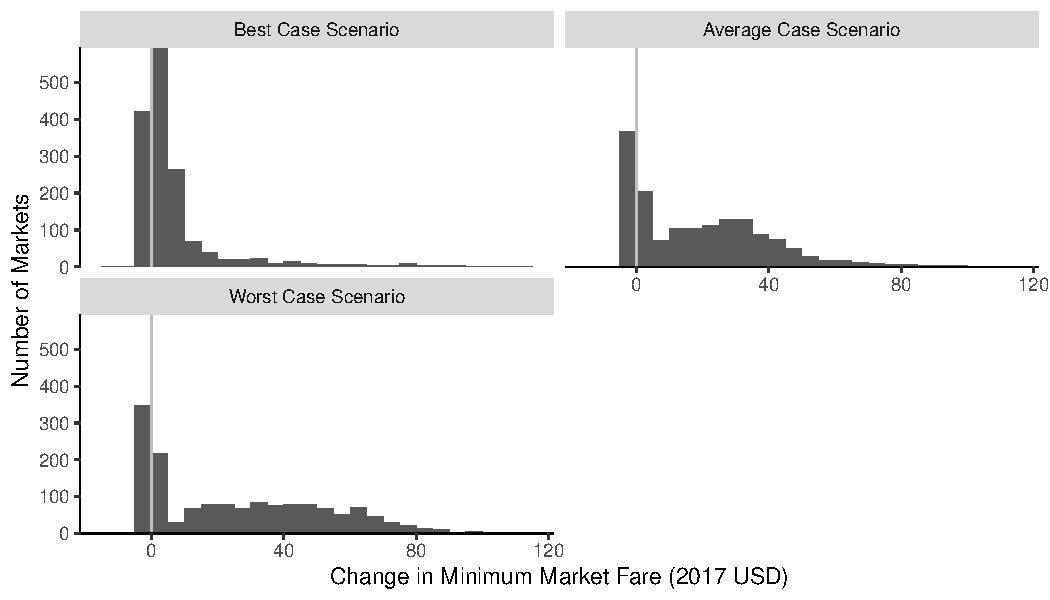
\includegraphics[width = \linewidth]{PrePandemic_Merger_Change_MinimumFare_Dist}
    \label{fig:PrePan_MinimumFare_Dist}
    \footnotesize{The mean change in markets' minimum fares is 7.25 (19.36) [26.15] in the best (average) [worst] case merger simulations respectively.}  
    \end{figure}    

    \begin{figure}
    \caption{Simulated Change in Post-Pandemic Minimum Market Fares}
    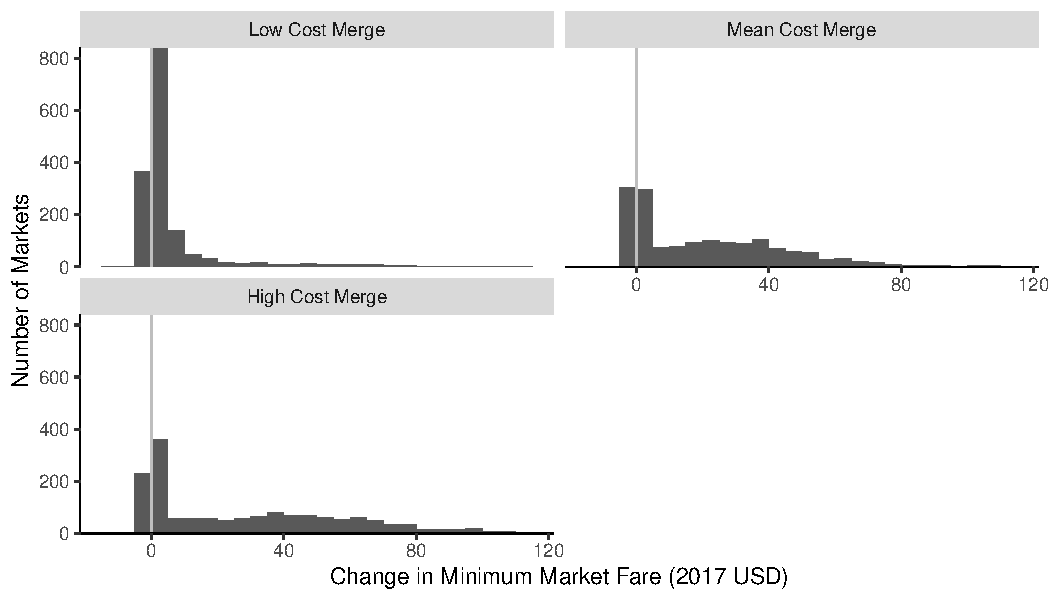
\includegraphics[width = \linewidth]{Merger_Change_MinimumFare_Dist}
    \label{fig:PostPan_MinimumFare_Dist}
    \footnotesize{The mean change in markets' minimum fares is 6.51 (21.45) [29.21] in the best (average) [worst] case merger simulations respectively.}  
    \end{figure}    

    Figures \ref{fig:PrePan_MinimumFare_Dist} and \ref{fig:PostPan_MinimumFare_Dist} graph the distribution of estimated minimum market fares for the pre-pandemic and post-pandemic periods. In the pre-pandemic (post-pandemic) period there exists roughly 300 (200) markets estimated to have decreases of under \$5 in the minimum market fare in all specifications. At the same time,  Importantly, these figures reveal the highly heterogeneous nature of the estimated changes under each simulation scenario, with the average case and best case scenarios having consistently highly dispersed predictions as to the change in the minimum market fares.   

  %  Now that the results on prices have been expounded upon, we can now turn our attention to how the simulations predict market concentration would change. Notably, as ultra-low cost airlines earn a significant amount of their income through axillary fares, which are not included within my dataset, estimation of market shares based on revenue are liable to understate these carriers within the market. As such, for these simulations, I calculate both an HHI calculated using market shares of airfare income as well as an HHI calculated using carrier shares of passengers within the market. These results are reported in Table  \ref{tab:HHI_Post}. Under every simulation model, I predict significant increases in market concentration under the passenger criterion, driven by an ascendant JetBlue. This is the opposite of the revenue shares criterion, which predicts significant declines in market concentration under the revenue criterion in all but the worst case scenarios. However, even under this more favorable metric, over 170 markets are still predicted to have increases about 100 points creating a structural presumption of illegality under the Department of Justice's 2023 merger guidelines. Overall, these results are consistent with a merger which would decrease consumer welfare in various markets while having effects that are pro-competitive at the national level.  

   %   \begin{table}
   %     \caption{Simulated Change in HHI}
   %     \label{tab:HHI_Post}
   %     \vspace{-15mm}
   %     \begin{center}
   %     
\begin{tabular}[t]{lrrrrrr}
\toprule
\multicolumn{1}{c}{ } & \multicolumn{3}{c}{Passenger Shares} & \multicolumn{3}{c}{Revenue Shares} \\
\cmidrule(l{3pt}r{3pt}){2-4} \cmidrule(l{3pt}r{3pt}){5-7}
 & Best & Average & Worst & Best & Average & Worst\\
\midrule
\addlinespace[0.3em]
\multicolumn{7}{l}{\textbf{Pre-Pandemic}}\\
\hspace{1em}$<$ 0 & 396 & 405 & 467 & 962 & 710 & 563\\
\hspace{1em}0 - 100 & 38 & 77 & 71 & 60 & 81 & 73\\
\hspace{1em}100 - 1000 & 347 & 541 & 531 & 350 & 510 & 508\\
\hspace{1em}1000 - 3000 & 382 & 447 & 409 & 153 & 227 & 356\\
\hspace{1em}3000 $<$ & 370 & 63 & 55 & 8 & 5 & 33\\
\midrule
\addlinespace[0.3em]
\multicolumn{7}{l}{\textbf{Post-Pandemic}}\\
\hspace{1em}$<$ 0 & 675 & 743 & 552 & 1338 & 1130 & 672\\
\hspace{1em}0 - 100 & 61 & 98 & 135 & 41 & 112 & 135\\
\hspace{1em}100 - 1000 & 221 & 400 & 589 & 150 & 259 & 565\\
\hspace{1em}1000 - 3000 & 262 & 275 & 272 & 25 & 53 & 182\\
\hspace{1em}3000 $<$ & 335 & 38 & 6 & 0 & 0 & 0\\
\midrule
\bottomrule
\end{tabular}

   %     \end{center}
   % \end{table}

    
  

  %  \subsubsection{Spirit Exit Simulation}
  % Following the failure of the merger with JetBlue to consummate, Spirit Airlines would file for chapter 11 bankruptcy protection. Within this section, I estimate the counterfactual pricing effects of Spirit exiting every market, which would occur should it ultimately need to change its filing to be for chapter 7 bankruptcy protection. 
    
	\section{Conclusion}
	\label{sec:Conclusion}
    The proposed JetBlue-Spirit merger would have seen the end of the largest ultra-low cost carrier in the United States had it not been blocked following suit by the Department of Justice in 2024. Through the use of a structural demand model, I estimate that this merger would have increased the average fare within the average market by roughly 4\% had it been completed in the post-pandemic period and negligibly impacted average market fares had it been completed during the pre-pandemic period.

    However, this result obscures a key insight into Spirit's role within the aviation industry, namely, that its presence within a market primarily impacts fares at the low end of the fare distribution due to its targeting cost-conscious consumers of air travel through unbundled fares. As such, it is critical to consider the change in the minimum market fares had the merger been completed. 

    Under even the assumptions most favorable to the pro-competitive effects of the merger, I estimate that over 35 markets in the pre-pandemic and post-pandemic periods would have seen fares increase by over \$60 had the merger been in effect. This finding aligns with the findings of the judge who considered the merger, who believed that the core consumer harm would have been for highly cost-conscious consumers at risk of being priced out of the market.

    Beyond the immediate findings of this paper regarding the anti-competitive effects of the JetBlue-Spirit merger, its results further our understanding of the role of maverick firms in differentiated product markets. Even in cases where these firms have minimal impact on average prices within a market, they may still significantly lower prices at the bottom end of the distribution of prices, allowing consumers to enter the market who would otherwise be unable to. 
    
	
	\pagebreak 
	\bibliography{airline} 
	\bibliographystyle{abbrvnat.bst}
	\FloatBarrier
	
\pagebreak 
\begin{appendices}
\setcounter{table}{0}
\setcounter{figure}{0}
\renewcommand{\thetable}{\Alph{section}\arabic{table}}
\renewcommand{\thefigure}{\Alph{section}\arabic{figure}}

	\section{Data Processing Methodology}
	\label{sec:DataProcessing}
	As detailed in Section \ref{sec:Data},	the Bureau of Transportation Statistics' Airline Origin and Destination Survey (DB1B) database was the primary data set used for this research. After compiling the DB1B into a single dataset for the years 2017 through the second quarter of 2023, some observations were excluded from the sample. Itineraries with fares lower than \$15 were excluded to remove air travel purchased through frequent flier rewards points (4.88\% of itineraries were excluded this way). Similarly, in line with prior work\footnote{such as \citet{berry_tracing_2010}}, itineraries with reported fares of over \$2,000 dollars were excluded to avoid erroneously recorded fares (0.08\% of itineraries were excluded this way). Beyond fares, itineraries were excluded from the sample if they had three or more layovers\footnote{A total of 0.03\% of itineraries were excluded this way.} or if they had a leg outside of the continental United States.\footnote{As noted in \citet{ciliberto_market_2021}, these flights receive subsidies from the United States Postal Service. As such, proper marginal cost recovery is infeasible while including them in the sample.} 
	
	Beyond this excluding of individual itineraries, additional filtering rules were placed on products and markets. All markets within the year 2020 and the first quarter of 2021 were dropped to avoid capturing the coronavirus pandemic induced decline in travel depicted in Figure \ref{fig:QuarterlyPass}. Furthermore, markets were excluded if they had fewer than 500 passengers fly within them, or had origin and destination airports within 150 miles. This restriction is in line with the past-literature (such as \citet{ciliberto_does_2014}) and serves to not only improve computational speed but also account for these markets featuring stronger substitutability to the outside good for travel. Finally, products with fewer than 100 passengers were excluded from the sample to avoid capturing irregular product offerings (2.50\% of itineraries were excluded this way). 
    	
	In calculating product shares, the total number of passengers of each product is ten times the number of passengers recorded as purchasing it within the DB1B as the DB1B is a 10\% sample. Following this, all airports not serving one of the hundred largest metropolitan statistical areas were dropped from the sample to improve computational speed. Notably, as both firms of interest within this paper focus on larger airport markets, this should have minimal impact on the results.  
	
	% Beyond the handling of data acquired from the DB1B, data on the daily spot price of jet fuel was acquired through the U.S. Energy Information Administration. This was averaged at the quarterly level. 
	
	As part of the handling of price data, prices were modified in two ways. For Spirit itineraries completed before 2020, fares had an additional \$22.99 times the number of trip legs added to them. This accounts for Spirit's additional usage fee placed on itineraries which were not booked in-person at the airport, and which the majority of consumers paid.\footnote{As documented in \citet{shrago_spirit_2024}, these fees were included in DB1B releases following 2020.} Furthermore,, prices were re-expressed in terms of 2017 United States dollars to account for inflation and allow for easier comparisons between the two sample periods.

    \FloatBarrier
    \section{Merger Pre-Approval Effects}
    \setcounter{table}{0}
    \setcounter{figure}{0}

    Historically, airline mergers have had effects on airfares before the completion of the merger. Within this section, I estimate the effects of the announcement of the merger on fares in markets served by both JetBlue and Spirit through a modified version of the model in \citet{goolsbee_how_2008} and \citet{fan_when_2020}. For carrier $c$ serving unidirectional route $r$ during quarter $q$, its average fare $y_{crq}$ is described by 

    \[\log(y_{crq}) = \sum_{i = - 4}^{4} \beta_{M,i}I[q = i] Merge_{c} + \sum_{i = - 8}^{4} \beta_{O,i}I[q = i] Other_{c}  + \mu_cr + \gamma X_{crq}+ \epsilon_{crq}\]

    where $I[q = i]$ is $1$ if $q = i$ and zero otherwise, $Merge_{c}$ is a dummy variable which is one if carrier $c$ is either JetBlue or Spirit, $Other_c$ is one if the carrier neither of the merging firms, $\mu_{cr}$ is carrier-route fixed effects, $X_{crq}$ is a vector of controls, and $\epsilon_{crq}$ is a random error term. As the Spirit-JetBlue merger was approved by Spirit's board in the third quarter of 2022, period $0$ is defined as the second quarter of 2022. Furthermore, quarters from the height of the coronavirus pandemic (2020 and the first quarter of 2021) are excluded. 

    \FloatBarrier
	\section{Merger Comments Analysis}
    \label{sec:NaturalLanguage}

    \setcounter{table}{0}
    \setcounter{figure}{0}


As part of the merger process, JetBlue and Spirit were required to file an application with the Department of Transportation for the transference of operating certificates from Spirit to the combined firm, to be effective after the completion of the merger. Members of the public were allowed to leave public comments on the regulatory filing. Within this section, I employ stance detection techniques to analyze these comments at scale. While these comments are largely irrelevant to the result of this particular merger (namely, that it would be rejected following a suit brought by the Department of Justice), the use of these comments was used as part of the two firms' attempt to get the public to approve of the merger.

Stance detection, in brief, is the task of detecting the position held by the author of a text regarding some topic. In this context, it is to determine if the author of a comment left on the regulatory filing supported or opposed the proposed JetBlue-Spirit merger. This context is particularly suitable for the use of modern machine learning models as focused and direct. Therefore, an unsupervised zero-shot model should be effective with minimal issues with trying to gauge potentially contradictory statements that could be found in a longer work. 

The stance detection problem should not be confused with that of the sentiment analysis problem. Sentiment analysis intends to capture the emotions expressed in a text rather than identify the emotions expressed within the text. As an example of how these differ, consider the comment ``Competition is good for a healthy economy."\footnote{This is an actual comment left on the regulatory docket.} Using a pre-trained sentiment detection model developed for analyzing financial sentiment data, FinBERT, \footnote{Model documentation is contained in \citet{araci_finbert_2019}.} this statement is judged to possess positive sentiment. However, it is correctly judged to oppose the merger by the stance detection model used for my analysis. Table \ref{tab:Sentiment_Stance_Table} details the breakdown of unique comments' assigned sentiments and stances. 

\begin{table}
    \caption{Sentiment and Stance - Unique Comments}
    \label{tab:Sentiment_Stance_Table}
    \vspace{-15mm}
    \begin{center}
    
\begin{tabular}[t]{llll}
\toprule
\multicolumn{1}{c}{Stance} & \multicolumn{3}{c}{Sentiment} \\
\cmidrule(l{3pt}r{3pt}){1-1} \cmidrule(l{3pt}r{3pt}){2-4}
 & Positive & Neutral & Negative\\
\midrule
Approves & 40 & 37 & 4\\
Disapproves & 5 & 387 & 227\\
\bottomrule
\end{tabular}

    \end{center}
        \vspace{-5mm}
    \footnotesize{Each cell includes the number of comments with the given stance and sentiment. Only unique comments are included within this table. }
\end{table}

This paper uses the pre-trained model documented in \citet{laurer_less_2024} to detect the stances of each comment left on the docket. Each comment is assessed for the probability that each comment agrees with the statements ``The author of this comment \{approves of, disagrees with\} the merger." As these statements are mutually exclusive, the probabilities assigned for each comment sum to 1. As documented in Figures \ref{fig:ProbabilityApprove} and \ref{fig:ProbabilityApprove_Unique}, most comments are strongly polarized, suggesting that the language model had little difficulty in assigning stances to comments. Looking over a sample of fifty unique comments, all are sorted as would be expected based on my understanding of the text. As such, I believe that this model is well suited for analyzing the public comments.  

	\begin{figure}
		\caption{Probability Comments Approve}
		\label{fig:ProbabilityApprove}
        \begin{center}
        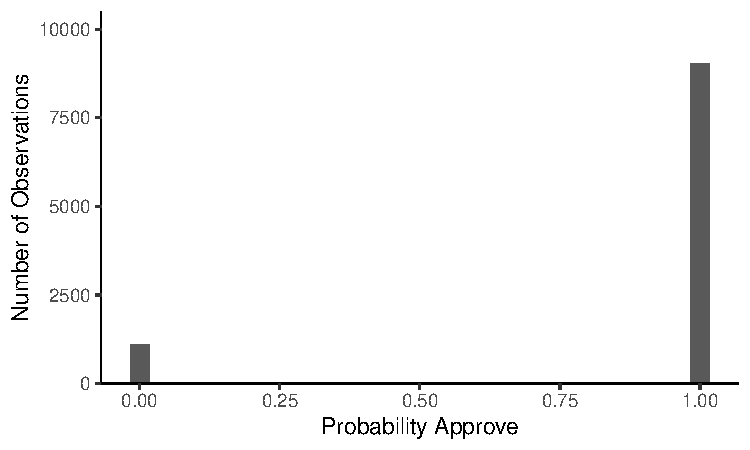
\includegraphics{05.Figures/stance_strength_graph}
        \end{center}
		\begin{minipage}{\textwidth} 
			{\footnotesize Data is sourced from the Department of Transportation regulatory filing regarding the JetBlue-Spirit merger (DOT-OST-2023-0024). ``Probability Approve" is the probability that a comment approves of the merger.} 
		\end{minipage}
	\end{figure}
	
	\begin{figure}
		\caption{Probability Comment Approves - Unique Comments Only}
		\label{fig:ProbabilityApprove_Unique}
        \begin{center}
            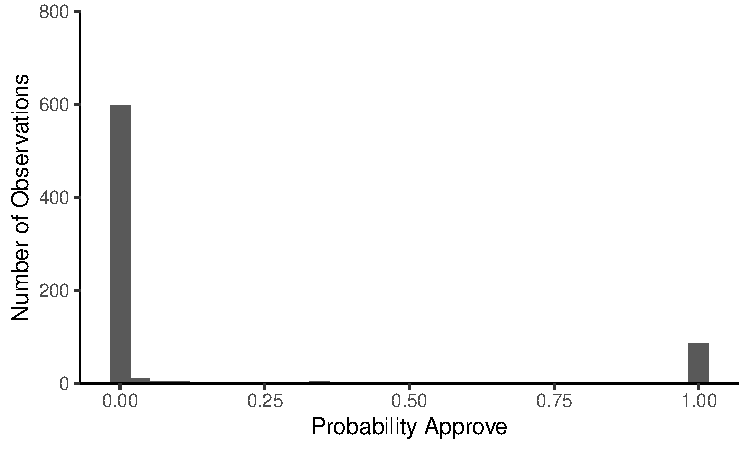
\includegraphics{05.Figures/stance_strength_unique.pdf}
        \end{center}
				\begin{minipage}{\textwidth} 
			{\footnotesize Data is sourced from the Department of Transportation regulatory filing regarding the JetBlue-Spirit merger (DOT-OST-2023-0024). ``Probability Approve" is the probability that a comment approves of the merger.} 
		\end{minipage}
	\end{figure}


Table \ref{tab:Stance_Summary} contains summary statistics for these comments. Most comments approve of the merger. However, this is driven by duplicate comments. \footnote{The exact legitimacy of these duplicate comments was a matter of some public debate, with some lawmakers alleging that they represented an "astroturf campaign" by the two merging firms falsely attributing them to employees \citep{birnbaum_elizabeth_2023}.}  The vast majority of unique comments, on the other hand, disapproved of the merger. On average, comments which approve of the merger are longer than those that disapprove. This table provides a helpful demonstration of the difference between the stance detection and sentiment detection problems -  the majority of disapproving comments expressed their views with neutral sentiment. Finally, the table documents the state of origin for the comments. 

\begin{table}[h]
    \caption{Stance Detection Summary Statistics}
    \label{tab:Stance_Summary}
    
\begin{tabular}[t]{llllll}
\toprule
 & Mean & (SD) & Minimum & Median & Maximum\\
\midrule
\addlinespace[0.3em]
\multicolumn{6}{l}{\textbf{All Comments}}\\
\hspace{1em}P(Approves) & 0.89 & (0.31) & 0 & 1 & 1\\
\hspace{1em}Approving Comment P(Approves) & 1 & (0.02) & 0.51 & 1 & 1\\
\hspace{1em}Disapproving Comment P(Approves) & 0.01 & (0.04) & 0 & 0 & 0.49\\
\hspace{1em}New York Comment & 0.14 & (0.35) & 0 & 0 & 1\\
\hspace{1em}Florida Comment & 0.35 & (0.48) & 0 & 0 & 1\\
\hspace{1em}Massachusetts Comment & 0.05 & (0.22) & 0 & 0 & 1\\
\hspace{1em}Puerto Rico Comment & 0.01 & (0.12) & 0 & 0 & 1\\
\midrule
\hspace{1em}Observations & 10185 &  &  &  & \\
\midrule
\addlinespace[0.3em]
\multicolumn{6}{l}{\textbf{Unique Comments}}\\
\hspace{1em}P(Approves) & 0.13 & (0.32) & 0 & 0 & 1\\
\hspace{1em}Approving Comment P(Approves) & 0.98 & (0.08) & 0.51 & 1 & 1\\
\hspace{1em}Disapproving Comment P(Approves) & 0.01 & (0.06) & 0 & 0 & 0.49\\
\hspace{1em}New York Comment & 0.06 & (0.24) & 0 & 0 & 1\\
\hspace{1em}Florida Comment & 0.07 & (0.26) & 0 & 0 & 1\\
\hspace{1em}Massachusetts Comment & 0.03 & (0.18) & 0 & 0 & 1\\
\hspace{1em}Puerto Rico Comment & 0 & (0) & 0 & 0 & 0\\
\midrule
\hspace{1em}Observations & 701 &  &  &  & \\
\midrule
\bottomrule
\end{tabular}

    \begin{minipage}{\textwidth} 
        {\footnotesize Data is sourced from the Department of Transportation regulatory filing regarding the JetBlue-Spirit merger  (DOT-OST-2023-0024). Comments have the stance with the highest probability assigned to them. This is the ``Stance Probability." Similarly, ``Sentiment Assigned Probability" is the sentiment with the highest  probability assigned to a comment by the language model. Comment length is in characters.} 
    \end{minipage}
\end{table}

Figure \ref{fig:CommentTimeline} plots the distribution of submitted comments on each day after the regulation was available for commenting upon. In the first twenty days, virtually every comment left on the docket supported the merger. Virtually every comment left on the docket after this period was opposed the merger. This may reflect asymmetry in the the resources available to JetBlue, Spirit, and anti-merger consumer welfare organizations.  

    \begin{figure}[h]
		\caption{Timeline of Submitted Comments}
		\label{fig:CommentTimeline}
        \begin{center}
    	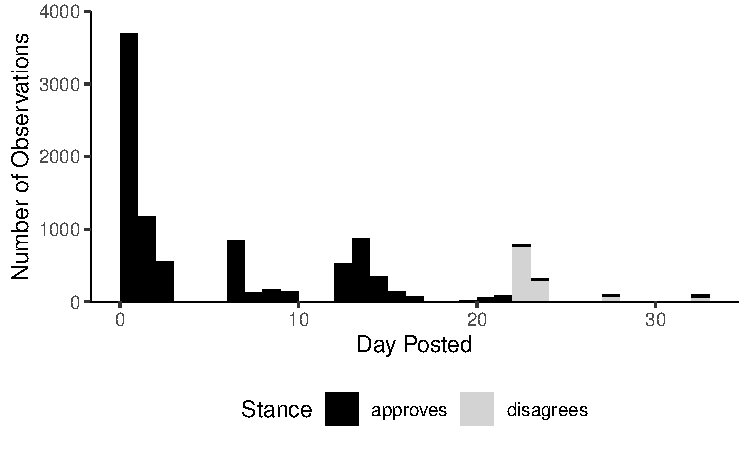
\includegraphics{stance_submission_timeline}
        \end{center}
		\begin{minipage}{\textwidth} 
			{\footnotesize Data is sourced from the Department of Transportation regulatory filing regarding the JetBlue-Spirit merger  (DOT-OST-2023-0024). Comments have the stance with the highest probability assigned to them.} 
		\end{minipage}
	\end{figure}
	
	
	\FloatBarrier
	\pagebreak
	\section{Additional Figures and Tables}	
    \setcounter{table}{0}
    \setcounter{figure}{0}


    \subsection{Additional Descriptive Figures and Tables: Aviation Industry}
    \begin{figure}[h]
        \caption{Distribution of Low-Cost and Ultra-Low Cost Carriers}
        \label{fig:LCC_Distribution}
        \begin{center}
    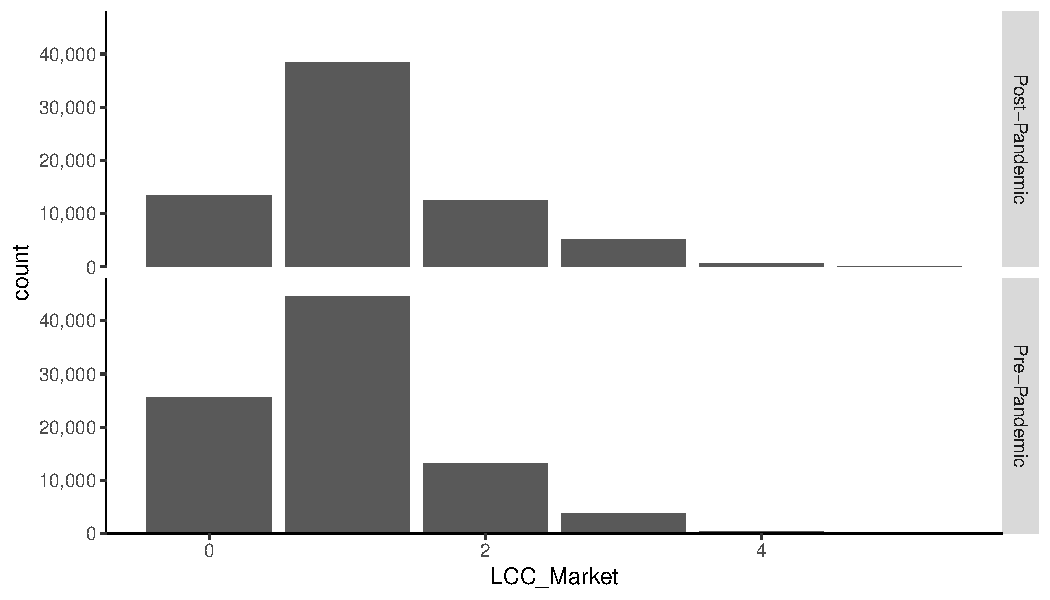
\includegraphics{05.Figures/LCC_Market_Graph.pdf}
        \end{center}
        \footnotesize{Each market is a Year-Quarter-Origin Airport-Destination Airport ordered quartet. Carriers included in the count of low-cost and ultra-low cost carriers are Southwest, JetBlue, Spirit, Frontier, and Allegiant.}
    \end{figure}
    \FloatBarrier
    
	\subsection{Additional Descriptive Figures and Tables: Northeast Alliance}
	 \begin{figure}
        \caption{Northeast Alliance Passenger Uptake}
        \label{fig:NEA_Uptake}
        \begin{center}
            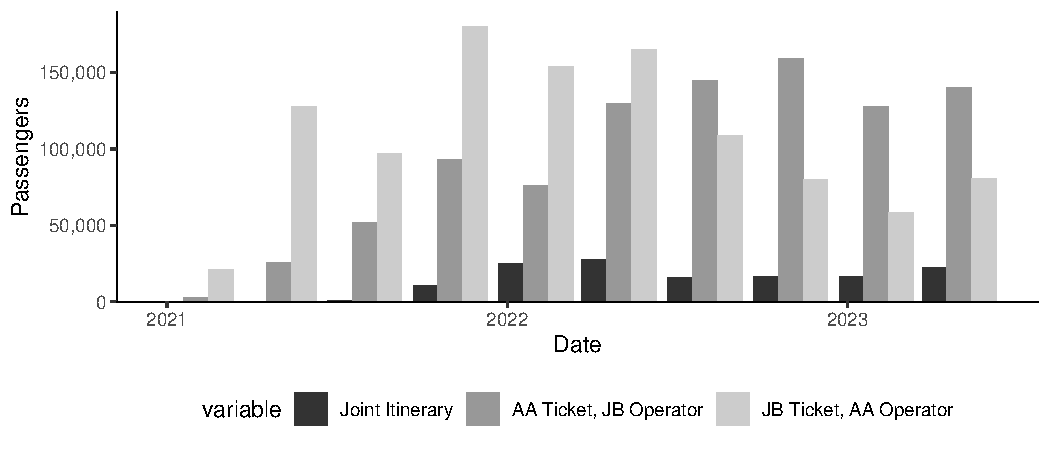
\includegraphics[width = \linewidth]{05.Figures/NEA_OperationsGraph}
        \end{center}
        \vspace{-8mm}
        \footnotesize{A joint itinerary is one in which both JetBlue and American Airlines operated flights on one or more legs of the unidirectional trip. The ticketing carrier collects fares and issues tickets, the operating carrier operates the flights. Itineraries are classified as an "AA Ticket, JB Operator" if the entire itinerary was issued by American Airlines and JetBlue operated at least one leg of the trip.}
    \end{figure}

\begin{landscape}
    \begin{table}
        \caption{NEA Codesharing Products}
        \label{tab:NEA_Codesharing_Table}
        \vspace{-15mm}
        \begin{center}
        
\begin{tabular}[t]{lrrrrrrrrrrr}
\toprule
 & 2021Q1 & 2021Q2 & 2021Q3 & 2021Q4 & 2022Q1 & 2022Q2 & 2022Q3 & 2022Q4 & 2023Q1 & 2023Q2 & 2023Q3\\
\midrule
\addlinespace[0.3em]
\multicolumn{12}{l}{\textbf{All Markets}}\\
\hspace{1em}JetBlue Only & 843 & 1375 & 1327 & 1374 & 1363 & 1583 & 1531 & 1456 & 1412 & 1562 & 1640\\
\hspace{1em}JetBlue American Required & 10 & 22 & 25 & 17 & 24 & 27 & 21 & 29 & 18 & 41 & 35\\
\hspace{1em}JetBlue-American Joint & 0 & 0 & 0 & 67 & 90 & 69 & 50 & 85 & 74 & 134 & 90\\
\hspace{1em}American Only & 4487 & 6728 & 7534 & 7351 & 7119 & 7596 & 8099 & 8338 & 7742 & 8173 & 8434\\
\hspace{1em}American JetBlue Required & 61 & 90 & 86 & 87 & 84 & 88 & 87 & 75 & 81 & 81 & 86\\
\hspace{1em}American-JetBlue Joint & 1 & 0 & 0 & 1 & 0 & 0 & 2 & 1 & 2 & 6 & 3\\
\addlinespace[0.3em]
\multicolumn{12}{l}{\textbf{Spirit Markets}}\\
\hspace{1em}JetBlue Only & 338 & 438 & 420 & 447 & 409 & 517 & 490 & 540 & 554 & 644 & 676\\
\hspace{1em}JetBlue American Required & 4 & 11 & 6 & 9 & 10 & 15 & 12 & 14 & 11 & 17 & 12\\
\hspace{1em}JetBlue-American Joint & 0 & 0 & 0 & 22 & 26 & 20 & 16 & 27 & 25 & 44 & 33\\
\hspace{1em}American Only & 1161 & 1491 & 1694 & 1849 & 1773 & 2012 & 2112 & 2340 & 2309 & 2563 & 2666\\
\hspace{1em}American JetBlue Required & 16 & 28 & 28 & 30 & 27 & 31 & 16 & 23 & 21 & 25 & 28\\
\hspace{1em}American-JetBlue Joint & 0 & 0 & 0 & 0 & 0 & 0 & 0 & 0 & 0 & 0 & 1\\
\bottomrule
\end{tabular}

        \end{center}
        \vspace{-5mm}
        \footnotesize{Each row indicates the number of products within a given quarter that belong to each classification. A "Firm Only" product is one in which the product had no codesharing flights included within it. A "JetBlue American Required" product is one in which all itineraries credited to the JetBlue for that quarter had all legs operated by American. A "JetBlue-American Joint" product is one where at least one leg was operated by each firm. A Spirit Market is one in which Spirit operated within it during the given quarter of interest. }
    \end{table}
\end{landscape}
    \begin{figure}[h]
        \caption{NEA: Overlapped Operating Routes}
        \label{fig:NEA_Operating}
        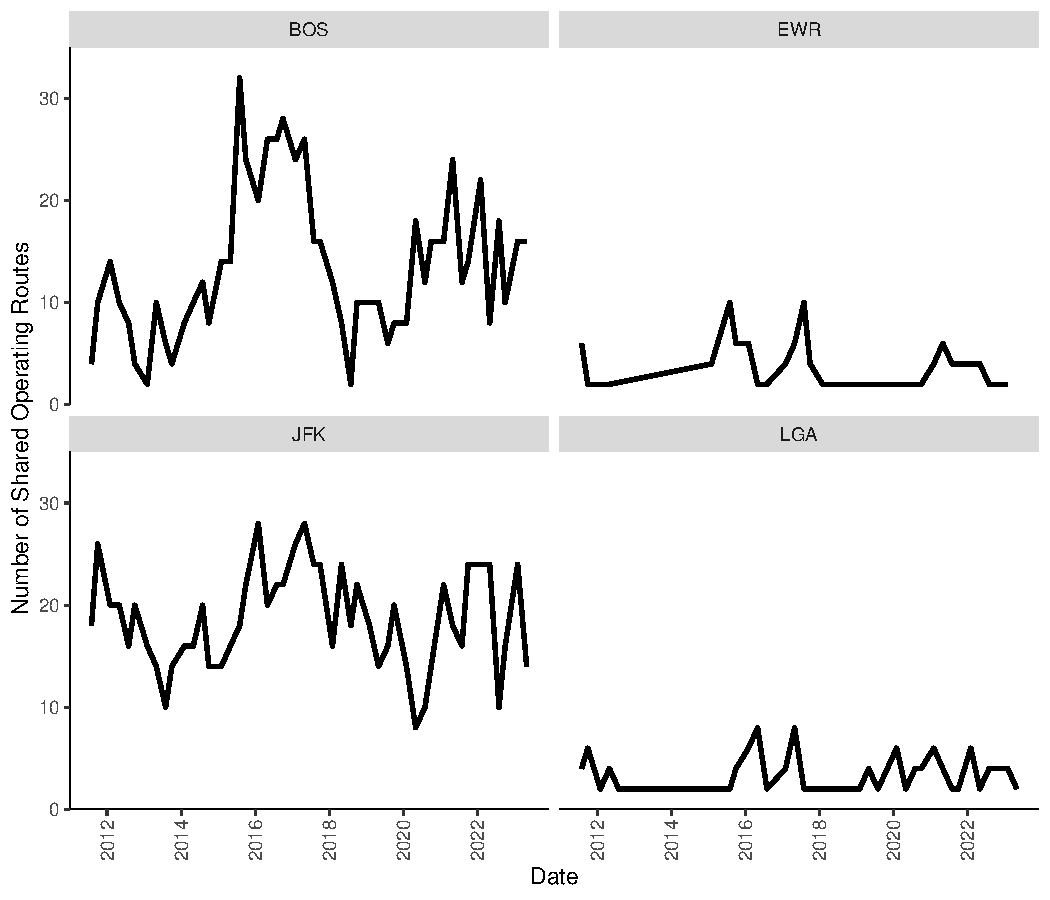
\includegraphics[width = \linewidth]{05.Figures/NEA_Operating_Graph.pdf}
        \footnotesize{Figure plots the number of routes operated by both JetBlue and American within a given quarter. The vertical line represents the start of the Northeast Alliance in January 2021.}
    \end{figure}

    \FloatBarrier\pagebreak

	\subsection{Descriptive Figures and Tables: JetBlue, Spirit}
	\begin{figure}[h]
	\caption{JetBlue, Spirit Fleet Size Over Time}
	\label{fig:Both_fleet}
	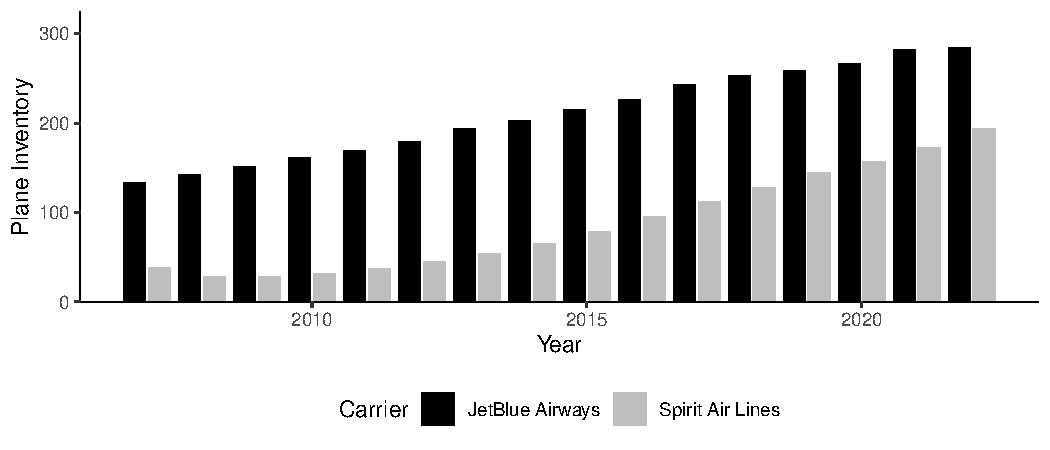
\includegraphics[width = \linewidth]{Both_Planes.pdf}
	\footnotesize{Source: B-43 Inventory Data. Each bar is the number of airplanes in a given firm's inventory within a given year.}
\end{figure}


\begin{table}[h]
		\caption{American, JetBlue Overlap at NEA Airports}
		\label{tab:NEA_Airport_Prescence}
        \vspace{-15mm}
        \begin{center}
         
\begin{tabular}[t]{rrrrrrrrr}
\toprule
\multicolumn{1}{c}{ } & \multicolumn{2}{c}{JFK} & \multicolumn{2}{c}{BOS} & \multicolumn{2}{c}{LGA} & \multicolumn{2}{c}{EWR} \\
\cmidrule(l{3pt}r{3pt}){2-3} \cmidrule(l{3pt}r{3pt}){4-5} \cmidrule(l{3pt}r{3pt}){6-7} \cmidrule(l{3pt}r{3pt}){8-9}
Year & Ticket & Operating & Ticket & Operating & Ticket & Operating & Ticket & Operating\\
\midrule
\addlinespace[0.3em]
\multicolumn{9}{l}{\textbf{Q1}}\\
\hspace{1em}2023 & 75.4 & 23.7 & 69.1 & 21.4 & 67.3 & 4.2 & 46.7 & 7.7\\
\hspace{1em}2022 & 77.0 & 29.7 & 75.0 & 29.1 & 73.9 & 8.9 & 47.6 & 8.3\\
\hspace{1em}2021 & 18.6 & 24.4 & 26.8 & 21.7 & 50.0 & 33.3 & 9.5 & 13.6\\
\hspace{1em}2019 & 22.4 & 23.3 & 22.9 & 20.0 & 8.1 & 6.7 & 0.0 & 0.0\\
\addlinespace[0.3em]
\multicolumn{9}{l}{\textbf{Q2}}\\
\hspace{1em}2023 & 70.0 & 15.9 & 63.1 & 22.2 & 68.3 & 5.4 & 46.7 & 7.7\\
\hspace{1em}2022 & 68.3 & 26.5 & 70.3 & 21.9 & 75.0 & 6.4 & 45.5 & 17.4\\
\hspace{1em}2021 & 57.7 & 21.1 & 57.4 & 28.6 & 27.3 & 7.4 & 28.6 & 13.6\\
\hspace{1em}2019 & 21.1 & 21.0 & 21.2 & 25.0 & 8.9 & 5.6 & 0.0 & 0.0\\
\addlinespace[0.3em]
\multicolumn{9}{l}{\textbf{Q3}}\\
\hspace{1em}2023 & 69.0 & 16.9 & 63.9 & 19.0 & 61.0 & 4.1 & 40.0 & 7.7\\
\hspace{1em}2022 & 73.8 & 21.9 & 73.8 & 24.2 & 75.9 & 6.4 & 57.1 & 7.1\\
\hspace{1em}2021 & 63.6 & 25.9 & 58.9 & 23.1 & 30.4 & 3.2 & 37.5 & 14.8\\
\hspace{1em}2019 & 19.6 & 20.3 & 21.6 & 21.6 & 8.9 & 5.6 & 0.0 & 0.0\\
\addlinespace[0.3em]
\multicolumn{9}{l}{\textbf{Q4}}\\
\hspace{1em}2022 & 72.1 & 25.4 & 66.1 & 21.1 & 69.8 & 2.0 & 46.7 & 7.7\\
\hspace{1em}2021 & 71.9 & 25.8 & 73.2 & 23.2 & 75.0 & 4.3 & 43.5 & 7.7\\
\hspace{1em}2019 & 15.3 & 17.5 & 22.0 & 19.2 & 6.8 & 5.4 & 0.0 & 0.0\\
\bottomrule
\end{tabular}

        \end{center}
                \vspace{-5mm}
		\footnotesize{Each cell is the percent of markets originating from the specified airport with both carriers present in the market as either the ticketing carrier or operating carrier. Ticketing carriers are responsible for buying and selling of tickets while the operating carrier handles flight operations. Data for the first quarter of 2021 should be interpreted cautiously as this was before widespread vaccination availability.}
\end{table}

\begin{figure}
	\caption{JetBlue, Spirit Airports - 2022}
	\label{fig:JBSpirit_Airports_2022}
	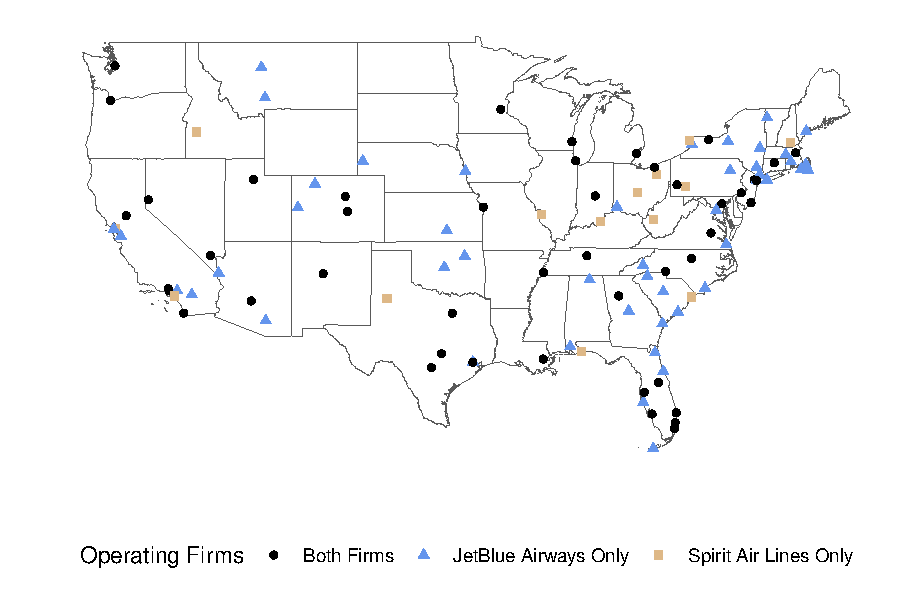
\includegraphics[width = \linewidth]{Map_Mainland_Both_2022.pdf}
	\footnotesize{Derived from DB1B Data. Beyond the United States mainland, both carriers operated in Puerto Rico.}
\end{figure}


	\begin{table}
		\caption{JetBlue and Spirit: Overlap Cities - 2022}
		\label{tab:KeyCities}
		
\begin{tabular}{lrrr}
\toprule
City & Firm Passengers & Total Passengers & Share\\
\midrule
Ponce, PR & 106320 & 106320 & 1.000\\
Aguadilla, PR & 251180 & 321170 & 0.782\\
San Juan, PR & 1848180 & 4149260 & 0.445\\
Boston, MA & 4262240 & 12136460 & 0.351\\
West Palm Beach/Palm Beach, FL & 919690 & 2960650 & 0.311\\
\addlinespace
Miami, FL & 5885260 & 19049140 & 0.309\\
Charlotte Amalie, VI & 155220 & 584450 & 0.266\\
New York, NY & 8243150 & 32401400 & 0.254\\
Hartford, CT & 596840 & 2358950 & 0.253\\
Orlando, FL & 4890200 & 19981730 & 0.245\\
\addlinespace
Fort Myers, FL & 964970 & 4577540 & 0.211\\
Detroit, MI & 1330090 & 7481070 & 0.178\\
Cleveland, OH & 567000 & 3537960 & 0.160\\
Richmond, VA & 235760 & 1474130 & 0.160\\
New Orleans, LA & 774190 & 4909390 & 0.158\\
\addlinespace
Las Vegas, NV & 2783710 & 18384770 & 0.151\\
Tampa, FL & 1371860 & 9955070 & 0.138\\
Pittsburgh, PA & 391900 & 3023570 & 0.130\\
Los Angeles, CA & 2839960 & 22400620 & 0.127\\
Philadelphia, PA & 844170 & 7694760 & 0.110\\
\bottomrule
\end{tabular}

		\footnotesize{Derived from DB1B Data. Cities are ordered by the combined share of passengers who used JetBlue or Spirit flights as a share of the total passengers departing from the city within 2022. Cities in which only one firm operates are excluded.}
	\end{table}

	
	\FloatBarrier
	
\FloatBarrier
    \subsection{Additional Merger Figures}
    \begin{table}
        \caption{Market Level Summary Statistics (By Competition Structure)}
        \label{fig:Market_Type_Summary}
                  \vspace{-15mm}
        \begin{center}
        
\begin{tabular}[t]{llllll}
\toprule
 & Mean & (SD) & Minimum & Median & Maximum\\
\midrule
\addlinespace[0.3em]
\multicolumn{6}{l}{\textbf{Pre-Pandemic}}\\
\addlinespace[0.3em]
\multicolumn{6}{l}{\textbf{Spirit Markets}}\\
\hspace{1em}\hspace{1em}Minimum Miles (1000s) & 1.3 & (0.61) & 0.18 & 1.14 & 2.81\\
\hspace{1em}\hspace{1em}Average Miles (1000s) & 1.35 & (0.66) & 0.18 & 1.19 & 4.39\\
\hspace{1em}\hspace{1em}Number of Firms & 4.8 & (1.37) & 1 & 5 & 9\\
\hspace{1em}\hspace{1em}Number of Products & 6.53 & (2.25) & 1 & 7 & 14\\
\hspace{1em}\hspace{1em}Number of Customers & 51859.49 & (48793.03) & 300 & 37600 & 360320\\
\hspace{1em}\hspace{1em}HHI & 8225.48 & (4382.4) & 1622.69 & 7360.39 & 56397.84\\
\midrule
\hspace{1em}\hspace{1em}Observations & 5941 &  &  &  & \\
\midrule
\addlinespace[0.3em]
\multicolumn{6}{l}{\textbf{JetBlue \& Spirit Markets}}\\
\hspace{1em}\hspace{1em}Minimum Miles (1000s) & 1.44 & (0.71) & 0.32 & 1.17 & 2.78\\
\hspace{1em}\hspace{1em}Average Miles (1000s) & 1.47 & (0.73) & 0.32 & 1.19 & 2.9\\
\hspace{1em}\hspace{1em}Number of Firms & 6.17 & (1.06) & 2 & 6 & 9\\
\hspace{1em}\hspace{1em}Number of Products & 8.51 & (2) & 3 & 8 & 15\\
\hspace{1em}\hspace{1em}Number of Customers & 80495.06 & (53421.42) & 1300 & 69680 & 344530\\
\hspace{1em}\hspace{1em}HHI & 6750.6 & (2646.51) & 1680.29 & 6247.49 & 17066.21\\
\midrule
\hspace{1em}\hspace{1em}Observations & 1533 &  &  &  & \\
\midrule
\addlinespace[0.3em]
\multicolumn{6}{l}{\textbf{Post-Pandemic}}\\
\addlinespace[0.3em]
\multicolumn{6}{l}{\textbf{Spirit Markets}}\\
\hspace{1em}\hspace{1em}Minimum Miles (1000s) & 1.32 & (0.6) & 0.18 & 1.22 & 2.81\\
\hspace{1em}\hspace{1em}Average Miles (1000s) & 1.37 & (0.63) & 0.18 & 1.26 & 2.92\\
\hspace{1em}\hspace{1em}Number of Firms & 5.11 & (1.24) & 2 & 5 & 8\\
\hspace{1em}\hspace{1em}Number of Products & 6.55 & (2.01) & 2 & 6 & 13\\
\hspace{1em}\hspace{1em}Number of Customers & 36898.62 & (37432.1) & 410 & 24260 & 214550\\
\hspace{1em}\hspace{1em}HHI & 7648.74 & (3855.01) & 1750.61 & 7023.19 & 19917.19\\
\midrule
\hspace{1em}\hspace{1em}Observations & 7569 &  &  &  & \\
\midrule
\addlinespace[0.3em]
\multicolumn{6}{l}{\textbf{JetBlue \& Spirit Markets}}\\
\hspace{1em}\hspace{1em}Minimum Miles (1000s) & 1.52 & (0.67) & 0.2 & 1.26 & 2.79\\
\hspace{1em}\hspace{1em}Average Miles (1000s) & 1.56 & (0.69) & 0.2 & 1.35 & 2.9\\
\hspace{1em}\hspace{1em}Number of Firms & 6.34 & (0.94) & 3 & 6 & 9\\
\hspace{1em}\hspace{1em}Number of Products & 8.78 & (1.78) & 3 & 9 & 14\\
\hspace{1em}\hspace{1em}Number of Customers & 73002.09 & (54873.21) & 2250 & 59070 & 261740\\
\hspace{1em}\hspace{1em}HHI & 6635.64 & (2769.53) & 1730.25 & 6207.7 & 17230.6\\
\midrule
\hspace{1em}\hspace{1em}Observations & 1554 &  &  &  & \\
\midrule
\bottomrule
\end{tabular}

        \end{center}
    \end{table}
    
    \begin{table}
        \caption{Pre-Pandemic Instrument Comparison Table}
        \label{tab:Instrument_Compare_Pre}
        \resizebox{\linewidth}{!}{%

\begin{tabular}{l c c c c c c c c c}
\toprule
 & Model 1 & Model 2 & Model 3 & Model 4 & Model 5 & Model 6 & Model 7 & Model 8 & Model 9 \\
\midrule
Price                       & $-0.42^{***}$ & $-4.97^{***}$ & $-0.18^{**}$  & $-0.18^{**}$  & $-2.12^{***}$ & $-0.14^{*}$   & $-2.09^{***}$ & $-2.28^{***}$ & $-2.23^{***}$ \\
                            & $(0.00)$      & $(0.09)$      & $(0.06)$      & $(0.06)$      & $(0.04)$      & $(0.06)$      & $(0.04)$      & $(0.03)$      & $(0.03)$      \\
Nesting                     & $0.55^{***}$  & $0.42^{***}$  & $-0.14^{***}$ & $-0.14^{***}$ & $0.12^{***}$  & $-0.14^{***}$ & $0.12^{***}$  & $0.18^{***}$  & $0.18^{***}$  \\
                            & $(0.00)$      & $(0.01)$      & $(0.01)$      & $(0.01)$      & $(0.01)$      & $(0.01)$      & $(0.01)$      & $(0.00)$      & $(0.00)$      \\
\midrule
Products in Market          &               & X             & X             & X             & X             & X             & X             & X             & X             \\
Gas Instruments             &               & X             &               &               & X             &               & X             &               & X             \\
Hub Interactions            &               &               & X             & X             & X             & X             & X             & X             & X             \\
Gandhi Instruments          &               &               &               &               &               & X             & X             & X             & X             \\
Exog Interactions           &               &               &               &               &               &               &               & X             & X             \\
Price Test                  &               & 101307.015    & 94273.624     & 94273.624     & 87736.444     & 94159.23      & 87480.095     & 78369.648     & 77831.661     \\
p-Value                     &               & 0             & 0             & 0             & 0             & 0             & 0             & 0             & 0             \\
Test of Over Identification &               & N/A           & 4187.14       & 4187.14       & 7279.16       & 4283.57       & 7526.31       & 11166.96      & 11605.17      \\
p-value                     &               & N/A           & 0             & 0             & 0             & 0             & 0             & 0             & 0             \\
R-Squared                   & $0.66$        & $-0.96$       & $0.32$        & $0.32$        & $0.27$        & $0.31$        & $0.28$        & $0.27$        & $0.28$        \\
Adj. R-Squared              & $0.66$        & $-0.96$       & $0.32$        & $0.32$        & $0.27$        & $0.31$        & $0.28$        & $0.27$        & $0.28$        \\
Mean Elasticity             & $-0.99$       & $-11.62$      & $-0.42$       & $-0.42$       & $-4.96$       & $-0.32$       & $-4.88$       & $-5.32$       & $-5.21$       \\
Median Elasticity           & $-1.00$       & $-11.74$      & $-0.42$       & $-0.42$       & $-5.01$       & $-0.33$       & $-4.93$       & $-5.37$       & $-5.27$       \\
Share Inelastic Products    & $0.51$        & $0.00$        & $1.00$        & $1.00$        & $0.00$        & $1.00$        & $0.00$        & $0.00$        & $0.00$        \\
Share JB Inelastic Products & $0.67$        & $0.00$        & $1.00$        & $1.00$        & $0.00$        & $1.00$        & $0.00$        & $0.00$        & $0.00$        \\
Share SP Inelastic Products & $0.88$        & $0.00$        & $1.00$        & $1.00$        & $0.00$        & $1.00$        & $0.00$        & $0.00$        & $0.00$        \\
Num. obs.                   & $307289$      & $307289$      & $307289$      & $307289$      & $307289$      & $307289$      & $307289$      & $307289$      & $307289$      \\
\bottomrule
\multicolumn{10}{l}{\scriptsize{$^{***}p<0.001$; $^{**}p<0.01$; $^{*}p<0.05$}}
\end{tabular}
        }
    \end{table}

\begin{table}
    \caption{Post-Pandemic Instrument Comparison Table}
    \label{tab:PostPand_Instrument_Compare}
    \resizebox{\linewidth}{!}{%
\begin{tabular}{l c c c c c c c c c}
\toprule
 & Model 1 & Model 2 & Model 3 & Model 4 & Model 5 & Model 6 & Model 7 & Model 8 & Model 9 \\
\midrule
Price                       & $-0.24^{***}$ & $-0.06$       & $1.50^{***}$  & $1.50^{***}$  & $0.01$        & $1.28^{***}$  & $-0.00$       & $-2.46^{***}$ & $-0.63^{***}$ \\
                            & $(0.00)$      & $(0.03)$      & $(0.16)$      & $(0.16)$      & $(0.03)$      & $(0.15)$      & $(0.03)$      & $(0.07)$      & $(0.03)$      \\
Nesting                     & $0.54^{***}$  & $-0.11^{***}$ & $-0.26^{***}$ & $-0.26^{***}$ & $-0.11^{***}$ & $-0.24^{***}$ & $-0.11^{***}$ & $0.15^{***}$  & $0.01^{**}$   \\
                            & $(0.00)$      & $(0.00)$      & $(0.01)$      & $(0.01)$      & $(0.00)$      & $(0.01)$      & $(0.00)$      & $(0.01)$      & $(0.00)$      \\
\midrule
Products in Market          &               & X             & X             & X             & X             & X             & X             & X             & X             \\
Gas Instruments             &               & X             &               &               & X             &               & X             &               & X             \\
Hub Interactions            &               &               & X             & X             & X             & X             & X             & X             & X             \\
Gandhi Instruments          &               &               &               &               &               & X             & X             & X             & X             \\
Exog Interactions           &               &               &               &               &               &               &               & X             & X             \\
Price Test                  &               & 77288.49      & 81853.459     & 81853.459     & 76910.107     & 81743.441     & 76883.509     & 66904.122     & 64536.553     \\
p-Value                     &               & 0             & 0             & 0             & 0             & 0             & 0             & 0             & 0             \\
Test of Over Identification &               & N/A           & 1269.2        & 1269.2        & 4165.87       & 1453.45       & 4271.75       & 7094.09       & 11604.74      \\
p-value                     &               & N/A           & 0             & 0             & 0             & 0             & 0             & 0             & 0             \\
R-Squared                   & $0.65$        & $0.34$        & $0.02$        & $0.02$        & $0.34$        & $0.09$        & $0.34$        & $0.16$        & $0.42$        \\
Adj. R-Squared              & $0.65$        & $0.34$        & $0.02$        & $0.02$        & $0.34$        & $0.08$        & $0.34$        & $0.16$        & $0.42$        \\
Mean Elasticity             & $-0.50$       & $-0.14$       & $3.19$        & $3.19$        & $0.02$        & $2.72$        & $0.00$        & $-5.22$       & $-1.34$       \\
Median Elasticity           & $-0.50$       & $-0.13$       & $3.14$        & $3.14$        & $0.02$        & $2.69$        & $0.00$        & $-5.15$       & $-1.33$       \\
Share Inelastic Products    & $1.00$        & $1.00$        & $0.02$        & $0.02$        & $1.00$        & $0.04$        & $1.00$        & $0.00$        & $0.23$        \\
Share JB Inelastic Products & $1.00$        & $1.00$        & $0.00$        & $0.00$        & $1.00$        & $0.01$        & $1.00$        & $0.00$        & $0.30$        \\
Share SP Inelastic Products & $1.00$        & $1.00$        & $0.11$        & $0.11$        & $1.00$        & $0.22$        & $1.00$        & $0.00$        & $0.84$        \\
Num. obs.                   & $265196$      & $265196$      & $265196$      & $265196$      & $265196$      & $265196$      & $265196$      & $265196$      & $265196$      \\
\bottomrule
\multicolumn{10}{l}{\scriptsize{$^{***}p<0.001$; $^{**}p<0.01$; $^{*}p<0.05$}}
\end{tabular}
    }
\end{table}

    \begin{figure}
        \caption{Distribution in Changes of Average Market Fare - Pre-Pandemic}
        \label{fig:AverageFare_ChangeDist_PrePandemic}
        \begin{center}
        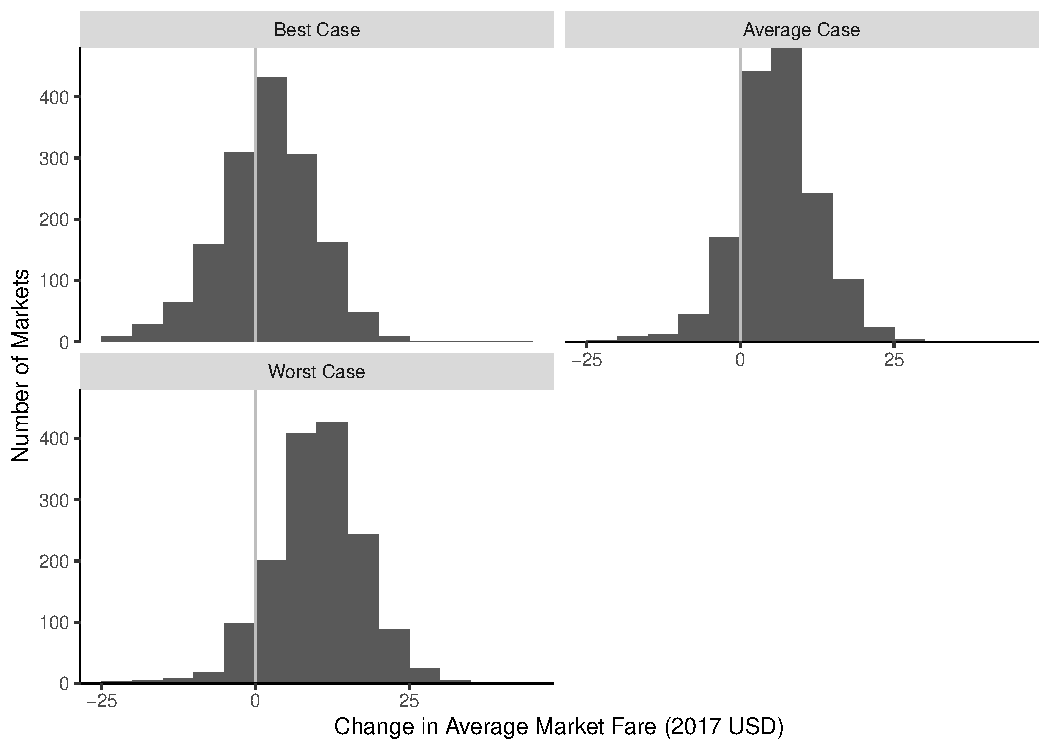
\includegraphics[width = \linewidth]{PrePandemic_Merger_Change_AverageFare_Dist.pdf}
        \end{center}
    \end{figure}

    \begin{figure}
        \caption{Distribution in Changes of Average Market Fare - Post-Pandemic}
        \label{fig:AverageFare_ChangeDist_PostPandemic}
        \begin{center}
        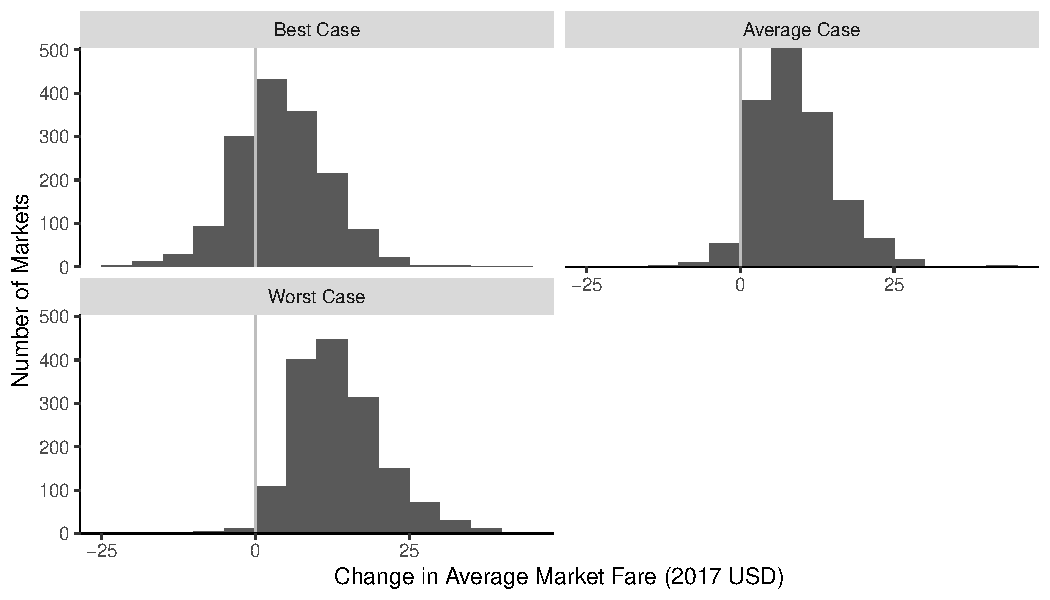
\includegraphics[width = \linewidth]{Merger_Change_AverageFare_Dist.pdf}
        \end{center}
    \end{figure}

    \begin{table}
        \caption{Change in Minimum Fare Available in Market (Percent)}
       \label{tab:MinimumPrice_Percent}
       \vspace{-15mm}
       \begin{center}
           
\begin{tabular}[t]{lrrrrrr}
\toprule
\multicolumn{1}{c}{ } & \multicolumn{3}{c}{Pre-Pandemic} & \multicolumn{3}{c}{Post-Pandemic} \\
\cmidrule(l{3pt}r{3pt}){2-4} \cmidrule(l{3pt}r{3pt}){5-7}
 & Best & Average & Worst & Best & Average & Worst\\
\midrule
$<$ 0 & 257 & 198 & 160 & 370 & 306 & 241\\
0-20 & 1171 & 704 & 619 & 1060 & 566 & 553\\
20-40 & 53 & 439 & 342 & 57 & 364 & 234\\
40-60 & 26 & 158 & 249 & 27 & 210 & 244\\
60-80 & 13 & 20 & 119 & 17 & 66 & 153\\
80 $<$ & 13 & 14 & 44 & 23 & 42 & 129\\
\bottomrule
\end{tabular}

       \end{center}
       \vspace{-5mm}
       \footnotesize{Products from markets without both JetBlue and Spirit present are excluded. The best case merger scenario is one in which the combined firm inherits the minimum average cost and greatest unobservables of each firm, the average case merger scenario has the combined JetBlue-Spirit inherit the average of the two firms' product characteristics, and the worst case scenario has the combined JetBlue-Spirit inherit the greatest marginal cost and lowest unobservables. A version of this table which reports the change in minimum fares in terms of 2017 dollars is included as Table \ref{tab:MinimumPrice}.}
    \end{table}
    \pagebreak 

    \FloatBarrier
    \section{Robustness Checks}
    \setcounter{table}{0}
    \setcounter{figure}{0}
    \subsection{Assumed Merger Efficiencies}
    \label{App:Efficiencies}
    In this section, I consider an alternative simulation method where for each case identified in the main text (Section \ref{sec:Analysis_Merger}), I additionally assume that the merged firm realizes efficiencies of either 5\% or 10\%. The results of this simulation for the 5\% case are reported in Table \ref{tab:Simulation_Price_5} and the results for the 10\% case in Table \ref{tab:Simulation_Price_10}. Minimum fare in market changes are reported in Tables \ref{tab:MinimumPrice_5} and \ref{tab:MinimumPrice_10}. 

        \begin{table}
        \caption{Simulated Price Effects of Merger with 5\% Efficiency Gain - Joint Markets}
        \label{tab:Simulation_Price_5}
                \vspace{-15mm}
        \begin{center}
         
\begin{tabular}[t]{lllllll}
\toprule
 & N & Mean & (SD) & Minimum & Median & Maximum\\
\midrule
\addlinespace[0.3em]
\multicolumn{7}{l}{\textbf{Pre-Pandemic}}\\
\addlinespace[0.3em]
\multicolumn{7}{l}{\textbf{Product Prices (100s, 2017 USD)}}\\
\hspace{1em}\hspace{1em}Observed & 12074 & 2.04 & (0.69) & 0.47 & 1.98 & 4.91\\
\hspace{1em}\hspace{1em}Best Case & 10106 & 2.06 & (0.67) & 0.46 & 2.01 & 5.08\\
\hspace{1em}\hspace{1em}Average Case & 10106 & 2.1 & (0.64) & 0.46 & 2.04 & 5.14\\
\hspace{1em}\hspace{1em}Worst Case & 10106 & 2.15 & (0.64) & 0.48 & 2.08 & 5.13\\
\addlinespace[0.3em]
\multicolumn{7}{l}{\textbf{Market Average Price}}\\
\hspace{1em}\hspace{1em}Observed & 1418 & 2.01 & (0.43) & 0.93 & 1.95 & \vphantom{1} 3.1\\
\hspace{1em}\hspace{1em}Best Case & 1418 & 1.7 & (0.61) & 0.79 & 1.52 & \vphantom{1} 3.44\\
\hspace{1em}\hspace{1em}Average Case & 1418 & 1.97 & (0.51) & 0.99 & 1.88 & \vphantom{1} 3.37\\
\hspace{1em}\hspace{1em}Worst Case & 1418 & 2 & (0.5) & 0.99 & 1.9 & \vphantom{1} 3.49\\
\addlinespace[0.3em]
\multicolumn{7}{l}{\textbf{\% Change Average Price}}\\
\hspace{1em}\hspace{1em}Best Case & 1418 & -16.62 & (17.31) & -54.03 & -18.81 & 31.39\\
\hspace{1em}\hspace{1em}Average Case & 1418 & -2.16 & (10.5) & -40.03 & -2.04 & 38.88\\
\hspace{1em}\hspace{1em}Worst Case & 1418 & -0.71 & (10.38) & -34.5 & -0.51 & 37.08\\
\addlinespace[0.3em]
\multicolumn{7}{l}{\textbf{Median Price}}\\
\hspace{1em}\hspace{1em}Observed & 1418 & 2.01 & (0.43) & 0.93 & 1.95 & 3.1\\
\hspace{1em}\hspace{1em}Best Case & 1418 & 1.7 & (0.61) & 0.79 & 1.52 & 3.44\\
\hspace{1em}\hspace{1em}Average Case & 1418 & 1.97 & (0.51) & 0.99 & 1.88 & 3.37\\
\hspace{1em}\hspace{1em}Worst Case & 1418 & 2 & (0.5) & 0.99 & 1.9 & 3.49\\
\midrule
\addlinespace[0.3em]
\multicolumn{7}{l}{\textbf{Post-Pandemic}}\\
\addlinespace[0.3em]
\multicolumn{7}{l}{\textbf{Product Prices  (100s, 2017 USD)}}\\
\hspace{1em}\hspace{1em}Observed & 13650 & 1.96 & (0.78) & 0.35 & 1.89 & 5.25\\
\hspace{1em}\hspace{1em}Best Case & 11496 & 2 & (0.77) & 0.4 & 1.93 & 5.34\\
\hspace{1em}\hspace{1em}Average Case & 11496 & 2.04 & (0.75) & 0.4 & 1.97 & 5.34\\
\hspace{1em}\hspace{1em}Worst Case & 11496 & 2.09 & (0.74) & 0.41 & 2.02 & 5.33\\
\addlinespace[0.3em]
\multicolumn{7}{l}{\textbf{Market Average Price}}\\
\hspace{1em}\hspace{1em}Observed & 1554 & 1.95 & (0.55) & 0.65 & 1.89 & \vphantom{1} 3.57\\
\hspace{1em}\hspace{1em}Best Case & 1554 & 1.68 & (0.67) & 0.6 & 1.64 & \vphantom{1} 3.61\\
\hspace{1em}\hspace{1em}Average Case & 1554 & 2.01 & (0.63) & 0.75 & 1.92 & \vphantom{1} 3.8\\
\hspace{1em}\hspace{1em}Worst Case & 1554 & 2.04 & (0.64) & 0.76 & 1.94 & \vphantom{1} 3.91\\
\addlinespace[0.3em]
\multicolumn{7}{l}{\textbf{\% Change Average Price}}\\
\hspace{1em}\hspace{1em}Best Case & 1554 & -15.49 & (18.28) & -60.19 & -13.02 & 38.4\\
\hspace{1em}\hspace{1em}Average Case & 1554 & 2.74 & (10.1) & -32.13 & 2.36 & 48.9\\
\hspace{1em}\hspace{1em}Worst Case & 1554 & 4.44 & (10.13) & -33.27 & 4.09 & 50.36\\
\addlinespace[0.3em]
\multicolumn{7}{l}{\textbf{Median Price}}\\
\hspace{1em}\hspace{1em}Observed & 1554 & 1.95 & (0.55) & 0.65 & 1.89 & 3.57\\
\hspace{1em}\hspace{1em}Best Case & 1554 & 1.68 & (0.67) & 0.6 & 1.64 & 3.61\\
\hspace{1em}\hspace{1em}Average Case & 1554 & 2.01 & (0.63) & 0.75 & 1.92 & 3.8\\
\hspace{1em}\hspace{1em}Worst Case & 1554 & 2.04 & (0.64) & 0.76 & 1.94 & 3.91\\
\bottomrule
\end{tabular}

        \end{center}
        \vspace{-5mm}
        \footnotesize{Products from markets without both JetBlue and Spirit present are excluded. The best case merger scenario is one in which the combined firm inherits the minimum average cost and greatest unobservables of each firm, the average case merger scenario has the combined JetBlue-Spirit inherit the average of the two firms' product characteristics, and the worst case scenario has the combined JetBlue-Spirit inherit the greatest marginal cost and lowest unobserveables. Each simulation additionally assumes that the merged firm's marginal cost additionally decreases by 10\%. Prices are in 2017 dollars.}

     \end{table}

     
        \begin{table}
        \caption{Simulated Price Effects of Merger with 10\% Efficiency Gain - Joint Markets}
        \label{tab:Simulation_Price_10}
                \vspace{-15mm}
        \begin{center}
         
\begin{tabular}[t]{lllllll}
\toprule
 & N & Mean & (SD) & Minimum & Median & Maximum\\
\midrule
\addlinespace[0.3em]
\multicolumn{7}{l}{\textbf{Pre-Pandemic}}\\
\addlinespace[0.3em]
\multicolumn{7}{l}{\textbf{Product Prices (100s, 2017 USD)}}\\
\hspace{1em}\hspace{1em}Observed & 12074 & 2.04 & (0.69) & 0.47 & 1.98 & 4.91\\
\hspace{1em}\hspace{1em}Best Case & 10106 & 2.05 & (0.67) & 0.46 & 2 & 5.08\\
\hspace{1em}\hspace{1em}Average Case & 10106 & 2.09 & (0.64) & 0.46 & 2.03 & 5.13\\
\hspace{1em}\hspace{1em}Worst Case & 10106 & 2.13 & (0.64) & 0.48 & 2.06 & 5.13\\
\addlinespace[0.3em]
\multicolumn{7}{l}{\textbf{Market Average Price}}\\
\hspace{1em}\hspace{1em}Observed & 1418 & 2.01 & (0.43) & 0.93 & 1.95 & \vphantom{1} 3.1\\
\hspace{1em}\hspace{1em}Best Case & 1418 & 1.67 & (0.61) & 0.77 & 1.47 & \vphantom{1} 3.44\\
\hspace{1em}\hspace{1em}Average Case & 1418 & 1.94 & (0.51) & 0.96 & 1.84 & \vphantom{1} 3.36\\
\hspace{1em}\hspace{1em}Worst Case & 1418 & 1.97 & (0.5) & 0.98 & 1.88 & \vphantom{1} 3.49\\
\addlinespace[0.3em]
\multicolumn{7}{l}{\textbf{\% Change Average Price}}\\
\hspace{1em}\hspace{1em}Best Case & 1418 & -18.2 & (17.76) & -54.99 & -20.68 & 31.36\\
\hspace{1em}\hspace{1em}Average Case & 1418 & -3.78 & (10.78) & -41.3 & -3.96 & 38.13\\
\hspace{1em}\hspace{1em}Worst Case & 1418 & -1.78 & (10.59) & -34.78 & -1.9 & 36.73\\
\addlinespace[0.3em]
\multicolumn{7}{l}{\textbf{Median Price}}\\
\hspace{1em}\hspace{1em}Observed & 1418 & 2.01 & (0.43) & 0.93 & 1.95 & 3.1\\
\hspace{1em}\hspace{1em}Best Case & 1418 & 1.67 & (0.61) & 0.77 & 1.47 & 3.44\\
\hspace{1em}\hspace{1em}Average Case & 1418 & 1.94 & (0.51) & 0.96 & 1.84 & 3.36\\
\hspace{1em}\hspace{1em}Worst Case & 1418 & 1.97 & (0.5) & 0.98 & 1.88 & 3.49\\
\midrule
\addlinespace[0.3em]
\multicolumn{7}{l}{\textbf{Post-Pandemic}}\\
\addlinespace[0.3em]
\multicolumn{7}{l}{\textbf{Product Prices  (100s, 2017 USD)}}\\
\hspace{1em}\hspace{1em}Observed & 13650 & 1.96 & (0.78) & 0.35 & 1.89 & 5.25\\
\hspace{1em}\hspace{1em}Best Case & 11496 & 1.99 & (0.78) & 0.4 & 1.91 & 5.34\\
\hspace{1em}\hspace{1em}Average Case & 11496 & 2.03 & (0.75) & 0.4 & 1.96 & 5.34\\
\hspace{1em}\hspace{1em}Worst Case & 11496 & 2.07 & (0.74) & 0.41 & 2 & 5.33\\
\addlinespace[0.3em]
\multicolumn{7}{l}{\textbf{Market Average Price}}\\
\hspace{1em}\hspace{1em}Observed & 1554 & 1.95 & (0.55) & 0.65 & 1.89 & \vphantom{1} 3.57\\
\hspace{1em}\hspace{1em}Best Case & 1554 & 1.64 & (0.65) & 0.59 & 1.6 & \vphantom{1} 3.53\\
\hspace{1em}\hspace{1em}Average Case & 1554 & 1.98 & (0.63) & 0.75 & 1.9 & \vphantom{1} 3.76\\
\hspace{1em}Worst Case & 1554 & 2.02 & (0.63) & 0.76 & 1.93 & \vphantom{1} 3.88\\
\addlinespace[0.3em]
\multicolumn{7}{l}{\textbf{\% Change Average Price}}\\
\hspace{1em}Best Case & 1554 & -17.46 & (18.33) & -61.06 & -15.42 & 37.34\\
\hspace{1em}Average Case & 1554 & 1.05 & (10.34) & -33.82 & 0.53 & 48.69\\
\hspace{1em}Worst Case & 1554 & 3.3 & (10.36) & -33.26 & 2.78 & 50.31\\
\addlinespace[0.3em]
\multicolumn{7}{l}{\textbf{Median Price}}\\
\hspace{1em}Observed & 1554 & 1.95 & (0.55) & 0.65 & 1.89 & 3.57\\
\hspace{1em}Best Case & 1554 & 1.64 & (0.65) & 0.59 & 1.6 & 3.53\\
\hspace{1em}Average Case & 1554 & 1.98 & (0.63) & 0.75 & 1.9 & 3.76\\
\hspace{1em}Worst Case & 1554 & 2.02 & (0.63) & 0.76 & 1.93 & 3.88\\
\bottomrule
\end{tabular}

        \end{center}
        \vspace{-5mm}
        \footnotesize{Products from markets without both JetBlue and Spirit present are excluded. The best case merger scenario is one in which the combined firm inherits the minimum average cost and greatest unobservables of each firm, the average case merger scenario has the combined JetBlue-Spirit inherit the average of the two firms' product characteristics, and the worst case scenario has the combined JetBlue-Spirit inherit the greatest marginal cost and lowest unobserveables. Each simulation additionally assumes that the merged firm's marginal cost additionally decreases by 10\%. Prices are in 2017 dollars.}

     \end{table}

    \begin{table}
        \caption{5\% Efficiency Case: Change in Minimum Fare Available in Market}
        \label{tab:MinimumPrice_5}
                \vspace{-15mm}
        \begin{center}
            
\begin{tabular}[t]{lrrrrrr}
\toprule
\multicolumn{1}{c}{ } & \multicolumn{3}{c}{Pre-Pandemic} & \multicolumn{3}{c}{Post-Pandemic} \\
\cmidrule(l{3pt}r{3pt}){2-4} \cmidrule(l{3pt}r{3pt}){5-7}
 & Best & Average & Worst & Best & Average & Worst\\
\midrule
$<$ 20 & 1407 & 928 & 772 & 1437 & 923 & 791\\
20-40 & 61 & 434 & 311 & 53 & 388 & 265\\
40-60 & 31 & 120 & 293 & 30 & 165 & 250\\
60-80 & 22 & 38 & 132 & 23 & 57 & 159\\
80 $<$ & 12 & 13 & 25 & 11 & 21 & 89\\
\bottomrule
\end{tabular}

        \end{center}
        \vspace{-5mm}
        \footnotesize{Products from markets without both JetBlue and Spirit present are excluded. The best case merger scenario is one in which the combined firm inherits the minimum average cost and greatest unobservables of each firm, the average case merger scenario has the combined JetBlue-Spirit inherit the average of the two firms' product characteristics, and the worst case scenario has the combined JetBlue-Spirit inherit the greatest marginal cost and lowest unobserveables. Each simulation additionally assumes that the merged firm's marginal cost additionally decreases by 5\%. Prices are in 2017 dollars.}
    \end{table}   

   \begin{table}
        \caption{10\% Efficiency Case: Change in Minimum Fare Available in Market}
        \label{tab:MinimumPrice_10}
                \vspace{-15mm}
        \begin{center}
            
\begin{tabular}[t]{lrrrrrr}
\toprule
\multicolumn{1}{c}{ } & \multicolumn{3}{c}{Pre-Pandemic} & \multicolumn{3}{c}{Post-Pandemic} \\
\cmidrule(l{3pt}r{3pt}){2-4} \cmidrule(l{3pt}r{3pt}){5-7}
 & Best & Average & Worst & Best & Average & Worst\\
\midrule
$<$ 20 & 1425 & 1032 & 820 & 1445 & 1021 & 814\\
20-40 & 49 & 372 & 319 & 47 & 353 & 285\\
40-60 & 28 & 89 & 265 & 34 & 130 & 254\\
60-80 & 19 & 28 & 107 & 18 & 32 & 137\\
80 $<$ & 12 & 12 & 22 & 10 & 18 & 64\\
\bottomrule
\end{tabular}

        \end{center}
        \vspace{-5mm}
        \footnotesize{Products from markets without both JetBlue and Spirit present are excluded. The best case merger scenario is one in which the combined firm inherits the minimum average cost and greatest unobservables of each firm, the average case merger scenario has the combined JetBlue-Spirit inherit the average of the two firms' product characteristics, and the worst case scenario has the combined JetBlue-Spirit inherit the greatest marginal cost and lowest unobserveables. Each simulation additionally assumes that the merged firm's marginal cost additionally decreases by 10\%. Prices are in 2017 dollars.}
    \end{table}  
    
  %  \subsection{Alternative Market Definition}
  %  In this section, I consider an alternative market definition where markets are defined by origin and destination metropolitan statistical areas rather than airports. Individual products within markets are defined by carrier, nonstop status, and airports traveled between. 
    
\end{appendices}
	
\end{document}